% chktex-file 8   en-dash compounds (supplier--customer) are correct academic usage
% chktex-file 12  interword spacing in captions/abbreviations is intentional
% chktex-file 13  intersentence spacing is a style choice for this document
% chktex-file 18  \MakeOuterQuote{"} is active in report_main.tex
% chktex-file 24  \label on own line after \chapter/\section is standard practice
\chapter{Introduction: The Silicon Backbone}
\label{chap:intro}
% ========================Introduction==============================
U.S.\ military power is bound by its access to semiconductors. Because the semiconductor supply chain is global, interdependent, and opaque beyond first-tier suppliers, the Department of Defense (DoD) faces hidden vulnerabilities that confer an advantage on actors capable of seeing and shaping these dependencies. This report addresses that problem by making those multi-tier dependencies visible and verifiable. It constructs a reproducible, auditable network of disclosed, predicted, and observed links that goes beyond vendor lists to reveal where operational risk actually resides.

The DoD is semiconductor-dependent for every phase of its mission, and that dependence converts supply-chain weaknesses into \emph{strategic risk}. Continuity shocks (lost output, schedule slip) slow force generation, reduce surge capacity, and degrade readiness; integrity failures (counterfeit or tampered devices) can deny or deceive effects at the point of use. Both dynamics alter deterrence, compress options in crisis, and lengthen campaign timelines. This report treats those outcomes not as hypotheticals but as consequences of the structure that analysis can identify and, with the right levers, change.

This section addresses structure rather than speculation. The analysis does not begin by estimating who might disrupt which node; instead, it first establishes what the DoD actually depends on. Concretely, the semiconductor ecosystem is modeled as a directed, multi-tier network with two intertwined layers: \emph{material flows} (from wafer to package to component) and \emph{information flows} (from IP blocks and design kits to firmware, test data, and process recipes). Entities are resolved, attributes (industry, geography, ownership) are attached, and edges are time-stamped, so the resulting map is auditable and suitable for analysis. Without a defendable map, discussions of risk, resilience, and assurance float free of the structure that governs them.

To keep the analysis precise, this report uses a risk language that distinguishes \emph{continuity} from \emph{integrity}. Continuity risk concerns output and schedule: shocks that reduce or delay production---natural hazards, cyber incidents, embargoes, service-contract interruptions, packaging bottlenecks---create calendar slip that erodes readiness. Integrity risk concerns trust and assurance: counterfeits, malicious modifications (including hardware Trojans), and tainted firmware can deceive or disable a system at the moment of need. The distinction is analytic, not absolute---risks often intertwine---but keeping them separate clarifies both mechanisms and remedies.

The sequencing of the analysis matters. \emph{Visibility precedes defense.} Probability estimates without structure are brittle; structure makes probability meaningful. A clear map of dependencies is the precondition for sensible priors, for targeted resilience measures (dual sourcing, buffers, qualification pathways) that address continuity, and for assurance measures (provenance, verification, device trust) that address integrity. ``the probability of disruption'' is defined conceptually but not directly estimated; the appropriate first task is illumination of the network the Department intends to defend.

The scope is bounded to the defense-relevant semiconductor network: firms and facilities as nodes; supplier, service, and information exchanges as directed edges; and attributes that matter for national security (industry activity, geographic footprint, ownership, and related features). Material and information flows are treated as first-class and interdependent. All data in this report are open-source or commercially licensed; no classified sources are used. The goal is a network map that is rigorous enough to analyze and transparent enough to inspect.

To address the visibility gap, this report uses a three-stage pipeline. \textbf{Disclosed:} a directed supplier graph is constructed from commercial and public sources, entities are resolved, and nodes are enriched with industry, geography, and ownership attributes. \textbf{Predicted:} missing links are treated as a supervised problem on a heterogeneous, time-aware graph, using leakage-safe evaluation and calibrated uncertainty to identify likely hidden tiers. \textbf{Observed:} shipment-based evidence derived from publicly available customs data (bills of lading) is layered to illuminate material flows between firms. These observations are not vendor-disclosed relationships; rather, they are event-level signals of inter-firm exchange used to corroborate or refine edges and to promote a subset of predictions to an \emph{observed} layer with explicit provenance and quality flags.

The section is organized as follows. Section~\ref{sec:framing-thesis} demonstrates how the modern U.S.\ military runs on chips, linking mission threads to specific device classes. Section~\ref{sec:chip-primer} provides a concise primer on chips to help non-specialist readers and technical audiences share vocabulary and concepts. Section~\ref{sec:manufacturing} outlines the semiconductor manufacturing process and walks the reader from design through wafer fabrication to assembly--test--packaging, translating process realities into calendar realities that matter for readiness. Section~\ref{sec:sc-network} reframes the industry as a directed multi-tier network with intertwined material and information flows, explaining why specialization and tacit know-how produce opacity below Tier-1. Section~\ref{sec:risk-classes} develops the continuity-versus-integrity risk taxonomy and links it to mission consequences. Section~\ref{sec:visibility-pipeline} formalizes the disclosed $\rightarrow$ predicted $\rightarrow$ observed pipeline, including the role of shipment-based observation in promoting predictions to observed edges. Section~\ref{sec:roadmap} closes with a roadmap for the remainder of the report and the policy translation that follows.

% ============Section 1.1 The U.S. Military Runs on Chips=====================
\section{The Modern U.S. Military Runs on Chips}
\label{sec:framing-thesis}

Semiconductor-based technologies fundamentally underpin modern U.S.\ military power. Over the past decade, government reports and policy analyses have documented how microelectronics permeate every facet of American defense. All major U.S.\ defense systems and platforms now rely on semiconductors for their performance, making chips as critical as ammunition or fuel to generate and sustain combat power \parencite{ch5_dod2022_supplychains,shivakumar_semiconductors_2022,national_academies_assured_2024}. This section establishes the military's deep dependence on microelectronics---from large platforms and mission systems down to individual warfighter gear---and highlights why secure access to semiconductors has become a strategic concern for U.S.\ readiness and national security.

Semiconductors are embedded in virtually every modern weapon platform and mission system fielded by the United States. Advanced microelectronics enable sensing, computing, communications, and control---the "brains" of platforms across air, land, sea, space, and cyberspace \parencite{ch5_dod2022_supplychains}. Erosion of access to key devices degrades platform modes, extends timelines, and restricts effects \parencite{TheWhiteHouse2021,national_academies_assured_2024}.

Modern combat aircraft are effectively flying computers: mission systems, flight controls, radar, and electronic warfare suites are based on specialized processors and custom chips, with key devices sourced from global foundries and advanced packaging ecosystems \parencite{shivakumar_semiconductors_2022,ch5_dod2022_supplychains}. The broader supply chain for advanced processors and sensors, including design, fabrication, and testing, links American airpower to overseas manufacturing nodes that are integral to performance and availability \parencite{shivakumar_semiconductors_2022}.

On the ground, ruggedized microelectronics drive fire control, active protection, navigation, and digital mission command; tactical radios, battle-management systems, and sensor networks are all powered by chips. Even logistics vehicles and command posts depend on electronics for situational awareness, communications, and routing functions that presume assured access to microprocessors, memories, trusted cryptographic elements, and timing devices \parencite{us_army_army_2025}.

At sea, naval radars and combat information centers integrate sensor-shooter chains through high-performance processors; undersea platforms rely on microelectronics in propulsion control, sonar processing, navigation, and weapons. In space, satellites for communications, positioning, navigation, and timing (PNT) and missile warning are hardened semiconductor systems in orbit, and continued access to microelectronics underwrites precision-guided munitions, hypersonic weapons, and space architectures \parencite{goodrich_dont_2025, national_security_administration_us_2016, national_academies_assured_2024}.

Across the cyber domain, encryption devices, servers, and data centers that tie the force together run on commercial semiconductors; AI-enabled tools ride cutting-edge processors, and losing access to them would erode advantages in all domains of warfare \parencite{NationalSecurityCommissiononArtificialIntelligence2021}. The operational network---secure communications, data transport, and edge computing---inherits the availability and cadence of the commercial semiconductor ecosystem \parencite{mondschein_securing_2022}.

Semiconductors have become fundamental building blocks of U.S.\ military power: they execute computing in mission systems, enable secure communications, process sensor data, and guide precision weapons. The deep integration of microelectronics into military hardware and infrastructure means that combat effectiveness now inherently relies on assured access to reliable chips \parencite{ch5_dod2022_supplychains, TheWhiteHouse2021}.

The dependence on semiconductors extends beyond exquisite platforms to small units and the individual warfighter. Infantry formations carry encrypted radios, data links, GPS receivers, night-vision and thermal sights, laser rangefinders, tablets, and small unmanned systems, each built on compact semiconductors and networked back to command and fires. The individual soldier has become a node in a microelectronics web: communications, navigation, sensing, and targeting now presume ruggedized chips at the edge \parencite{us_army_army_2025,national_academies_assured_2024}.

Modern tactical radios are effectively specialized computers; battlefield networking, waveform agility, and encryption are chip-enabled functions. Night-vision goggles and thermal weapon sights incorporate semiconductor image sensors and micro-displays, enabling low-light and thermal imaging capabilities for helmets and weapon mounts. Squad-level tablets and navigational aids integrate satellite receivers, inertial sensors, and processors to provide maps, blue-force tracking, and fire-control data in compressed timelines. The path is toward greater digitization: small unmanned systems, augmented-reality displays, and wearable sensors at the squad level all expand the microelectronic footprint of the dismounted force \parencite{program_executive_office_soldier_project_2025}. These improvements raise lethality and survivability, but they also mean that even basic combat skills now assume the availability of microelectronic devices.

Precision-guided munitions and expendable systems are built around microelectronics. Air-delivered weapons such as Joint Direct Attack Munition (JDAM) and Small Diameter Bombs, ground-based fires such as guided rockets and artillery shells, and a wide spectrum of missiles and loitering munitions all contain seekers, inertial sensors, embedded processors, GPS receivers, and power-management components, turning explosives into computers that fly. Even artillery and mortar rounds increasingly use electronic fuzes or guidance kits governed by on-board chips \parencite{Hoehn2021,pergolizzi_pgk_2010}.

This architecture has two implications. First, wartime consumption scales microelectronics demand: high-intensity conflict expends precision systems at tempo, so \emph{sustainment is inseparable from chip availability} \parencite{Hoehn2021, jones_empty_2023}. Second, replenishment timelines can be paced by component access rather than steel or energetics; scarcity and obsolescence redesigns have slowed select replenishment efforts, underscoring how component access gates production \parencite{mondschein_securing_2022, jones_empty_2023}. Munitions output is gated by semiconductors as much as by explosives or casings.

Because U.S.\ forces are so dependent on microelectronics, the security of microelectronic supply chains has become a strategic readiness concern. The DoD's microelectronics supply chain is global and interdependent, with a large share of manufacturing, assembly, and test capacity offshore, and with critical dependencies concentrated in East Asia \parencite{U.S.GovernmentAccountabilityOffice2025,TheWhiteHouse2021}. The Department of Defense has formally identified microelectronics as a defense-critical supply-chain vulnerability. It has elevated semiconductor access to the same tier of concern as fuel or ammunition for readiness planning \parencite{U.S.Congress2022,vergun_industry_2024,ch5_dod2022_supplychains}.

Risk scenarios turn on structural exposure. The world's most advanced chips are produced by a handful of foundries in Asia, creating potential single points of failure; a significant disruption would reverberate through U.S.\ defense production and degrade fielded capability \parencite{shivakumar_semiconductors_2022,jones_empty_2023}. A large-scale shock to semiconductor supply would constrain readiness and delay force generation, even without a single platform being destroyed in combat, because calendar effects in chip production propagate directly into program timelines \parencite{NationalSecurityCommissiononArtificialIntelligence2021,ch5_dod2022_supplychains}. This strategic exposure exists before the first shot: if the value chain is not visible and secure, the vulnerability is already in place.

Integrity risk compounds continuity risk. Counterfeit or compromised components can create hidden failure modes and exploitation paths at the moment of need, which is why the Department has pursued trusted and assured microelectronics and selective on-shoring for sensitive devices \parencite{U.S.GovernmentAccountabilityOffice2012,U.S.GovernmentAccountabilityOffice2016,Annett2025, vergun_industry_2024}. The policy response---spanning the CHIPS and Science Act, the Microelectronics Commons hubs, and DARPA-aligned prototyping efforts---aims to reduce both continuity and integrity risks over time \parencite{U.S.Congress2022,lopez_dod_2023,mondschein_securing_2022}.

Having established that modern U.S.\ military power is bounded by assured access to specific classes of microelectronics, the report now turns to a concise technical primer that defines what these devices are and how they work. The next section introduces microelectronic device families (CPU, GPU, FPGA, ASIC), memory types, and the basic behavior of transistors in digital logic so that later claims about design, fabrication, assembly, testing, and packaging rest on a shared technical footing.

% =================Section 1.2 Chip Primer===================
\section{Chip Primer: What a Chip Is and How It Works}
\label{sec:chip-primer}

A "chip" is a tiny, patterned crystal that lets a system sense the world, compute on data, store information, and move that information to other components. In a smartphone, a camera sensor converts light into electrical signals, a processor processes those signals into images, memory stores photos and code, and wired/wireless interfaces shuttle data to the screen or to the network. Defense systems do the same four things at platform scale (radar or radio frequency (RF) front-ends sense; a mission computer computes; memory stores and tracks mission data; a data link moves information across the force). Throughout this primer, a four-function lens---sense, compute, store, move---organizes the discussion: semiconductors give us the controllable material foundation, integrated circuits combine analog interfaces with digital logic, memories retain state, and interconnects ferry bits between engines of computation \parencite{sze_physics_2007,smith_microelectronic_2015,rabaey_digital_2003,jacob_memory_2008}.

These chips are built from semiconductor materials whose current-carrying ability can be tuned. Metals conduct freely, and insulators hardly conduct at all; a semiconductor sits between them because electrons must cross a small but finite band gap to move from bound states to conducting states \parencite{ashcroft_solid_1976}. In silicon, that gap is small enough that temperature, electric fields, or trace dopants (intentional impurities) can dramatically change conductivity, creating n-type regions rich in electrons and p-type regions rich in "holes." By placing n- and p-type regions next to each other and applying voltages, engineers make structures whose current can be turned on and off at will---the basis for switching, logic, and memory \parencite{sze_physics_2007,pierret_semiconductor_1996, neamen_semiconductor_1997,sharma_solid_2013}. Silicon dominates digital logic and memory because it can be manufactured on an immense scale with stable properties. At the same time, compound semiconductors, such as gallium arsenide and gallium nitride, provide superior high-frequency and high-power performance for radar, electronic warfare, and power electronics \parencite{morkoc_handbook_2008,baliga_fundamentals_2019}.

With a controllable material in hand, the next ingredient is the switch: the transistor. In the most common form, the metal-oxide-semiconductor field-effect transistor (MOSFET), a voltage applied to a tiny gate electrode creates an electric field in a channel between a source and drain. With the gate high, the channel conducts (the switch is "on"), and with the gate low, it blocks current (the switch is "off"). Those two stable states map naturally to binary 1 and 0, so vast networks of MOSFETs implement logic, memory, and control. Modern logic uses complementary pairs---complementary metal-oxide-semiconductor (CMOS)---so that static power is near zero and energy is spent primarily when gates switch, which is why chips can toggle billions of times per second without melting down \parencite{razavi_design_2001}. Scaling has made these switches extraordinarily small and fast (picosecond- to nanosecond-scale transitions), allowing billions of transistors to coexist on a single die and to act in concert as arithmetic units, registers, and interconnects. For the purpose of this analysis, the mental model is simple: a chip is a city of coordinated on/off gates; computation is the choreography of their switching; and performance follows from how quickly, how predictably, and how efficiently those gates can be driven \parencite{taur_fundamentals_2009,weste_cmos_2011,rabaey_digital_2003}.

From individual switches, manufacturers build integrated circuits (ICs): complete electronic subsystems patterned onto single-crystal silicon and cut into individual dies \parencite{sze_physics_2007}. On each chip, millions to billions of transistors work together \parencite{weste_cmos_2011}. Digital circuitry treats voltages as two stable levels and composes transistors into logic gates, arithmetic units, registers, and processors \parencite{rabaey_digital_2003}. Analog circuitry manipulates continuous voltages and currents to amplify, filter, generate, or condition real-world signals \parencite{smith_microelectronic_2015, razavi_fundamentals_2008, rabaey_digital_2003}. Mixed-signal ICs place the two side by side so that sensing and actuation occur near the logic that interprets and controls them \parencite{pelgrom_analog--digital_2017}. In practice, mixed-signal chips co-locate analog-to-digital converters (ADCs) and digital-to-analog converters (DACs) with low-noise amplifiers, oscillators, and power-management blocks on the same die as digital processing, thereby reducing latency, noise pickup, and energy consumption \parencite{kester_data_2005}. Silicon remains the dominant material for dense digital logic and memory, while analog, radio frequency (RF), and precision-timing blocks impose constraints that careful mixed-signal layout and device choice address so a single IC can sense, digitize, compute, and interface efficiently at scale \parencite{lee_design_2004,razavi_fundamentals_2008}.

With the physics and circuit foundations in place, the discussion shifts to the chip families that carry the workload. In practice, modern electronics rely on a small set of recurring chip types---general-purpose processors, massively parallel accelerators, reconfigurable logic, fixed-function engines, and several kinds of memory---combined in different proportions depending on the job. Labels vary by vendor, but the underlying roles are stable across architectures and generations \parencite{hennessy_computer_2012,rabaey_digital_2003}.

The first family of devices is the central processing unit (CPU). A CPU is the general-purpose "do-anything" chip that runs software \parencite{patterson_computer_2018}. It reads a list of instructions, following steps one after another as a recipe. A CPU retrieves the next instruction, decodes it, executes it, and keeps track of its position in the program via a program counter \parencite{harris_digital_2022}. Because it loops through this cycle billions of times per second, it responds quickly to control-intensive tasks: on a laptop, that means opening an app or moving a cursor; on a fighter jet mission computer, it means coordinating sensors, displays, and radios \parencite{patterson_computer_2018}. Modern CPUs go faster by executing multiple steps of different instructions simultaneously (pipelining) and by exploiting instruction-level parallelism. They also keep frequently used data in small, fast static random-access memory (SRAM) caches near the cores, so that they do not constantly wait on main memory \parencite{hennessy_computer_2012,weste_cmos_2011,rabaey_digital_2003}. When data must come from farther away in dynamic random-access memory (DRAM), performance often stalls, classically referred to as the memory wall, so real-world CPU speed depends as much on the memory hierarchy and data movement as on the raw core speed \parencite{jacob_memory_2008,wulf_hitting_1995}. This combination of flexibility and fast control is why CPUs sit at the center of most systems, orchestrating the specialized chips around them \parencite{patterson_computer_2018}.

The next device family is the graphics processing unit (GPU). A GPU is a highly parallel mathematical engine that executes the same short program on multiple data points in parallel. In everyday terms, it draws your screen, renders games, and speeds up photo and video filters---most phones and many laptops include a GPU for exactly these reasons \parencite{nickolls_gpu_2010}. In a system, the central processing unit (CPU) stages the work. It sends the GPU a small "kernel" to run across thousands of lightweight threads, which is why GPUs excel at operations that repeat across pixels in an image or numbers in a matrix \parencite{nickolls_gpu_2010, nickolls_scalable_2008}. That same pattern is what makes GPUs so useful for artificial intelligence and machine learning (AI/ML): training and inference are dominated by matrix multiplications and convolutions that benefit from running the same operation across many data elements in parallel \parencite{ieee_electronics_packaging_society_heterogeneous_2024,nickolls_gpu_2010}. Sustained speed depends on how fast data reaches those threads. Modern accelerators pair the compute die with high-bandwidth memory (HBM) and use advanced packaging to place memory close to compute; when bandwidth or locality is insufficient, throughput collapses as threads stall waiting on data \parencite{ieee_electronics_packaging_society_heterogeneous_2024,jacob_memory_2008}. GPUs, therefore, shine when the work is highly parallel and batched, and a small setup delay (moving data and launching kernels) is acceptable, and they are less suited to hard real-time, microsecond-class determinism, where even modest scheduling or transfer delays matter more than raw arithmetic rate \parencite{patterson_computer_2018,nickolls_gpu_2010}.

The next device family is the field-programmable gate array (FPGA). An FPGA is a reconfigurable chip: after fabrication, a designer loads a bitstream that turns a blank fabric of logic blocks and routing into a custom hardware circuit for the intended task \parencite{hauck_reconfigurable_2008}. Instead of running instructions like a CPU or launching kernels like a GPU, an FPGA becomes the data path the designer specifies, allowing it to stream data through a fixed pipeline with very low and predictable latency, useful for sensor interfacing, software-defined radio, fast encryption, and other timing-critical functions \parencite{hauck_reconfigurable_2008}. FPGAs often deliver true parallelism by having many stages operate at once, and include static random-access memory (SRAM) on the chip, dedicated digital signal processing (DSP) slices, and high-speed I/O to keep data flowing \parencite{hauck_reconfigurable_2008}. The trade-off is development effort and absolute efficiency: a well-designed application-specific integrated circuit (ASIC) can outperform an FPGA in speed and energy for the same fixed function, but loses the ability to be updated in the field \parencite{kuon_measuring_2006}. In practice, defense systems use FPGAs when they need hardware-speed, deterministic behavior, and the option to reprogram logic as algorithms and waveforms evolve \parencite{hauck_reconfigurable_2008}.

The next device family is the application-specific integrated circuit (ASIC). An ASIC is a custom chip designed to perform a single task extremely well: rather than running general-purpose software, its logic is hard-wired at fabrication to implement a fixed function, such as an encryption engine, a radar pulse-compression pipeline, or an inference core for a trained neural network. Because every transistor is placed for a purpose, ASICs can achieve higher speed and far better energy efficiency than reconfigurable or general-purpose devices running the same algorithm, at the cost of flexibility \parencite{kuon_measuring_2006}. Design and verification take time and money (non-recurring engineering). Once the chip is built, its behavior is essentially frozen, which is why programs choose ASICs when requirements are stable, volumes justify the investment, or size-weight-power (SWaP) constraints demand maximum efficiency \parencite{weste_cmos_2011,patterson_computer_2018}. Recent roadmaps underscore how specialization and heterogeneous integration (placing dedicated accelerators alongside CPUs and memory, often through advanced packaging) have become a primary path to performance as conventional scaling slows \parencite{neisser_international_2021}. In defense systems, the result is pragmatic: when a workload is well understood and mission-critical---e.g., cryptography, high-rate signal processing, or real-time target recognition---an ASIC can deliver the required throughput and power savings that other devices cannot, while less settled or evolving functions remain on CPUs, GPUs, or field-programmable gate arrays \parencite{patterson_computer_2018,kuon_measuring_2006}.

The last core family is memory, which holds code and data close enough to compute to enable work to proceed at speed. Systems use a hierarchy because no single memory type is fast, large, and persistent simultaneously. Static random-access memory (SRAM) is very fast and predictable and sits on the processor die as a cache, but it is volatile and expensive per bit. Dynamic random-access memory (DRAM) provides the large main memory that programs use; it is volatile and slower than SRAM because each bit must be refreshed, but it offers much higher density and lower cost per bit. Non-volatile memory, such as Flash, retains contents without power and stores firmware, keys, logs, and bulk data, but it is much slower to access and update than DRAM. In practice, performance is bounded by the distance to the data: the processor runs quickly only when the required bytes are already in nearby SRAM, and it stalls when it must fetch from farther-away DRAM or storage. This classic memory wall arises from latency and bandwidth limits in the hierarchy \parencite{jacob_memory_2008,wulf_hitting_1995}. Modern designs mitigate this with multiple cache levels, wide buses, and packaging that places memory physically closer to the compute. Still, the basic trade-offs remain: SRAM for speed, DRAM for capacity, Flash for persistence, and system throughput set according to the efficiency with which data can be moved when needed \parencite{patterson_computer_2018,rabaey_digital_2003}.

Having established the material, the switch, and the main chip families, the discussion now shifts from what chips are to how they work. The focus narrows to the mechanics of computation---logic and state, the instruction cycle, and the movement of data through a memory hierarchy---because real performance and reliability depend as much on these dynamics as on raw transistor counts. Understanding this execution model lays the groundwork for the next section on manufacturing and, later, why packaging and supply chains translate directly to risk for the Department of Defense.

Digital chips perform two functions repeatedly: they compute with logic, and they remember with state. A logic gate is a tiny circuit that applies a simple rule to its inputs; for example, an AND gate outputs 1 only when both inputs are 1. By wiring many gates together, a chip performs arithmetic and makes decisions on streams of 0s and 1s \parencite{rabaey_digital_2003,harris_digital_2022}. To carry results from one step to the next, the chip uses state elements---latches and flip-flops---which hold bits long enough for the next operation to begin \parencite{rabaey_digital_2003,harris_digital_2022}. Most designs are synchronous, meaning a shared clock acts as a metronome so that all storage elements update in step, and the logic between them has a fixed time to settle \parencite{weste_cmos_2011}. Long tasks are partitioned into pipelines by inserting additional registers between logic blocks. That turns a single long step into several short ones, so different parts of many operations can be in progress simultaneously, as in an assembly line. The result is higher throughput, even if a single item still takes several stages to finish \parencite{patterson_computer_2018}.

At the core of a processor is the instruction cycle. The chip reads the next instruction from memory on the program counter (PC), determines what work it requires, performs that work on its arithmetic and control hardware, and then writes any result back before advancing the PC to the next instruction \parencite{harris_digital_2022}. Some instructions perform arithmetic or comparisons; others load data from memory into on-chip registers or store register contents back to memory; branch and jump instructions change the PC, allowing programs to make decisions and loop \parencite{patterson_computer_2018}. Modern designs overlap these steps, so several instructions are in different stages at once, an assembly line called pipelining, but the programmer's view remains the same: fetch, decode, execute, and repeat \parencite{hennessy_computer_2012}. Because each step touches memory differently, the real speed depends on how quickly instructions and data arrive: registers and on-chip caches reply in a few cycles, while trips to dynamic random-access memory (DRAM) can cost tens to hundreds of cycles \parencite{jacob_memory_2008}.

Engineers address this by employing multiple cache levels, smarter prefetching, wider on-chip interconnects, and physically moving memory closer to compute. Recent roadmaps emphasize advanced packaging---2.5D/3D stacking and high-bandwidth memory placed beside or above the compute die---to reduce the distance and energy per access \parencite{ieee_electronics_packaging_society_heterogeneous_2024}. Performance is co-determined by compute and data movement, so where bytes live and how quickly they reach the logic that needs them often matters as much as the raw speed of the cores \parencite{jacob_memory_2008,patterson_computer_2018}.

Some missions prioritize latency and determinism over raw arithmetic, while others prioritize throughput above all else; this is why different chips exist. When a system must react in tightly bounded microseconds, stabilizing a control surface, closing a guidance loop, or executing an electronic warfare (EW) countermeasure, the safest path is dedicated hardware with predictable timing, which is why field-programmable gate arrays (FPGAs) and, for stable functions, application-specific integrated circuits (ASICs) dominate at the edge \parencite{shivakumar_semiconductors_2022,kuon_measuring_2006}. By contrast, when the task is to push large volumes of uniform math, filter a wide image, correlate many signals, or run a neural network, throughput wins, and graphics processing units (GPUs) or fixed accelerators deliver far more results per second by running the same operation across many data elements in parallel \parencite{nickolls_scalable_2008}. Central processing units (CPUs) remain the orchestrators: they coordinate devices, handle irregular control flow, and step in where logic is branchy or small but urgent, yet their ultimate speed is still bounded by memory and data movement \parencite{patterson_computer_2018,jacob_memory_2008}. When a system must guarantee bounded latency, deterministic hardware (FPGA or ASIC) is the correct choice; when throughput is the priority, a GPU or fixed accelerator delivers far more results per second; and CPUs manage, sequence, and fill the gaps between them \parencite{hauck_reconfigurable_2008,kuon_measuring_2006,nickolls_gpu_2010}.

Many defense systems are first limited by size, weight, and power (SWaP). Small satellites, unmanned aerial vehicles, and soldier-carried gear must deliver effects within tight energy budgets and minimal cooling. Hence, the right choice is the chip that does the most work per watt and consumes the fewest joules to move data \parencite{patterson_computer_2018}. That is why fixed-function application-specific integrated circuits (ASICs) and carefully designed field-programmable gate arrays (FPGAs) show up at the edge: for a stable algorithm or well-defined pipeline, they beat general-purpose processors in efficiency while meeting strict timing \parencite{kuon_measuring_2006,hauck_reconfigurable_2008}. RF and high-power front ends add a materials dimension: gallium nitride (GaN) and gallium arsenide (GaAs) provide the voltage handling and frequency performance needed for modern radar and electronic warfare, complementing silicon logic and memory \parencite{baliga_fundamentals_2019,morkoc_handbook_2008, razavi_rf_1998}. Packaging also matters: advanced 2.5D/3D integration and high-bandwidth memory (HBM) place memory close to compute, cutting access energy and delay \parencite{ieee_electronics_packaging_society_heterogeneous_2024, jedec_jesd238_hbm3_2022}. In practice, SWaP, RF physics, packaging proximity, and the assurance parts---secure elements for keys, precision oscillators for time, and non-volatile memory for code and logs---often dictate what a mission can credibly field, not peak arithmetic rates \parencite{razavi_fundamentals_2008,us_department_of_commerce_defense_2009}.

First, a chip is built from a controllable material (the semiconductor) that allows us to carve transistors as switches and connect them into integrated circuits that sense, compute, store, and move information. Second, different device families make explicit trade-offs: flexibility (CPU), parallel throughput (GPU), deterministic timing and reconfigurability (FPGA), fixed-function efficiency (ASIC), and a memory hierarchy whose "distance to data" often sets the limit. Third, real performance and reliability are co-determined by compute and data movement, which is why advanced packaging (placing memory and chiplets close to compute in 2.5D/3D stacks) now matters as much as transistor counts \parencite{ieee_electronics_packaging_society_heterogeneous_2024}.

The next section will explore how chips are made, from design through wafer fabrication to assembly, test, and packaging. It shows why those process steps have long, coupled calendars and qualification bottlenecks. Understanding this manufacturing reality explains where multi-tier, often hidden dependencies originate and motivates the approach used to make them visible and verifiable in the DoD-relevant semiconductor network \parencite{national_science_and_technology_council_national_2024,us_department_of_commerce_defense_2009}.

% ===========Section 1.3 From Sand to Systems: How Chips Are Made============
\section{From Sand to Systems: How Chips Are Made}
\label{sec:manufacturing}

Semiconductor manufacturing is at the center of a global industry that now exceeds \$630 billion in annual sales \parencite{semiconductor_industry_association_2025_2025}. A single chip can require nearly 1{,}400 process steps and may cross dozens of international borders before it is finished \parencite{khan_semiconductor_2021,sia_fcc_filing_2021}. This section explains the flow from inputs to finished parts and sets up the detailed walk-through that follows.

Figure~\ref{fig:fig_chip_production_chart} summarizes the manufacturing flow in three broad categories: design, wafer fabrication, and assembly, test, and packaging (ATP) \parencite{khan_semiconductor_2021,varas_strengthening_2021}. Design turns specifications into layout by using electronic design automation, core IP, and foundry process design kits to generate the mask data that defines every device and wire \parencite{palma_growing_2022,weste_cmos_2011}. Wafer fabrication repeats a few operations with extreme precision: deposition, lithography, etch, clean, and inline metrology, with implants and anneals as needed---to build transistors and interconnect layer by layer \parencite{irds_lithography_technical_working_group_international_2023,irds_factory_integration_technical_working_group_international_2023}. ATP finishes known-good die into reliable components through singulation, die attach, wirebond or flip-chip interconnect, encapsulation, and electrical test, with advanced packaging now adding 2.5D and 3D integration where performance demands it \parencite{ieee_electronics_packaging_society_heterogeneous_2024}.

% =========================
% Figure: Chip Production Chart
% =========================
\begin{figure}[h]
  \centering
  \caption[\textit{The Semiconductor Supply Chain}]
  {\textit{The Semiconductor Supply Chain}}
  \label{fig:fig_chip_production_chart}

  % Graphic
  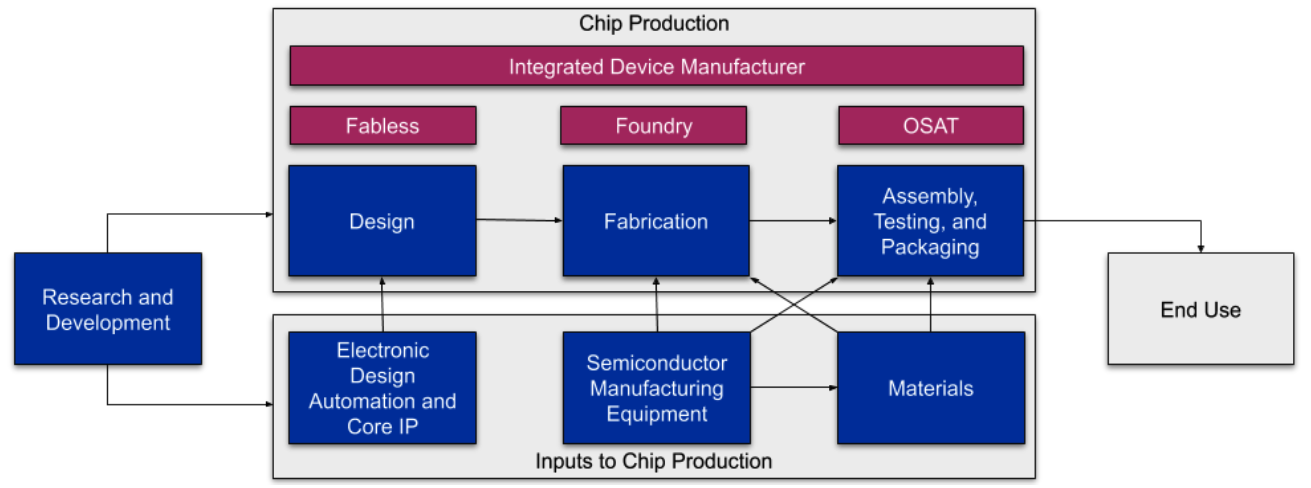
\includegraphics[width=\linewidth]{report/figures/fig_1.1_chip_production_chart.png}
    \captionsetup{justification=raggedright,singlelinecheck=false}
        \caption*{\footnotesize \textit{Note}. Production is organized into design, wafer fabrication, and assembly, test, and packaging (ATP), supported by production inputs: electronic design automation (EDA) and core IP, semiconductor manufacturing equipment (SME), and materials, with R\&D underpinning all stages. Business models include integrated device manufacturers (IDMs), fabless designers, foundries, and OSATs. Adapted from CSET, "The Semiconductor Supply Chain: Assessing National Competitiveness," 2021 \parencite{khan_semiconductor_2021}.}
\end{figure}

The first phase of the manufacturing process, design, turns a functional specification into a layout, a precise map of the shapes that will become transistors on silicon. Teams use electronic design automation (EDA) software, core IP blocks, and a foundry process design kit (PDK) to do this work \parencite{kahng_vlsi_2011,weste_cmos_2011}. The PDK is the foundry's rulebook and model set. It defines allowed line widths and spacings, device options, and electrical models that the tools use to predict timing, power, and reliability. Core IPs are pre-designed, pre-verified blocks---such as processor cores, memory controllers, and interfaces---that speed development and reduce risk \parencite{varas_strengthening_2021,khan_semiconductor_2021}. The main output is mask data---the layout files a mask shop uses to make photomasks (reticles). A photomask is a plate that carries the circuit pattern. The lithography tool uses it as a template to expose that pattern onto the wafer. Design also produces sign-off reports that show the chip meets the foundry's limits across operating corners. With verified layouts and mask data in hand, manufacturing begins on the wafers that will carry these patterns \parencite{kahng_vlsi_2011,weste_cmos_2011}.

The second phase of the manufacturing process is fabrication. Chips start as sand. Quartz is refined to metallurgical-grade silicon and then to electronic-grade polysilicon, the ultra-pure feedstock for crystals \parencite{us_geological_survey_mineral_2024,van_zant_microchip_2014}. In a crystal puller, the silicon is melted in a quartz vessel. A small seed crystal touches the melt and is slowly pulled and rotated so that its atoms line up with those of the melt. The result is a single-crystal cylinder---an ingot---that is sliced, ground, lapped, and polished into mirror-flat 200 or 300~mm wafers with tight control of thickness, flatness, and surface roughness \parencite{van_zant_microchip_2014,nishi_handbook_2007}. Many products add a thin, high-quality silicon layer on the surface to improve device uniformity. Some use a silicon-on-insulator structure, which places a buried insulator under the active silicon, suppressing unwanted current paths \parencite{nishi_handbook_2007}. These steps depend on subordinate resources that run continuously in the background. Fabs and wafer plants consume ultrapure water in large volumes, rely on high-purity gases and carefully filtered slurries and pads for polishing, and operate in cleanrooms that keep particles at extremely low levels \parencite{van_zant_microchip_2014,noauthor_iso_2015}. The energy and material footprint at this stage is significant, which is why contamination control and inspection are emphasized before the wafers reach device processing \parencite{williams_17kg_2002, van_zant_microchip_2014, irds_factory_integration_technical_working_group_international_2023}.

With verified layouts and mirror-flat wafers in hand, production moves to the cleanroom (Figure~\ref{fig:wafer_fabrication_process}). Wafers cycle through a repeating loop that builds each layer in turn: thin films are deposited or grown; the circuit image is transferred in lithography; unwanted material is etched away; surfaces are cleaned; and inline metrology checks that dimensions and alignment stay on target. Where needed, dopants and thermal anneals set device properties, and subsequent passes form the metal interconnects that link billions of transistors. Modern products can involve hundreds, or even more than a thousand, such steps over several weeks. The key point is that front-end fabrication is a long, tightly coupled sequence. Each stage depends on the accuracy of the last stage and on factory-integration choices such as scheduling, tool matching, and data feedback \parencite{sze_physics_2007, van_zant_microchip_2014, irds_factory_integration_technical_working_group_international_2023, may_fundamentals_2006}.

Once the wafer is cut and polished, the factory builds a stack of ultra-thin films that will become the raw material for devices. Bare silicon is given a controlled oxide skin, a few hundred nanometers of silicon dioxide grown in a furnace, thereby providing a clean, insulating starting surface. Additional layers are then deposited in sealed tools that feed high-purity gases and vapors (e.g., silane or ammonia) to form thick, precisely controlled dielectrics and conductors; later metal layers will serve as the wiring between transistors \parencite{van_zant_microchip_2014,nishi_handbook_2007}. Finally, the wafer is spin-coated with photoresist. This syrup-like material spreads into a uniform film only a fraction of a micron thick and is gently baked to set it. This is the paint that the lithography step will expose. Throughout, the fab runs on a steady background of ultrapure water, high-purity gases, and particle-free cleanrooms, so these films are uniform and free of defects; thickness and roughness are controlled to the nanometer scale because any defect here will print into every layer above it \parencite{noauthor_iso_2015,van_zant_microchip_2014}.

With the wafer prepared, the factory prints one layer of the circuit at a time (Figure~\ref{fig:lithography_process}). A photomask (reticle) holds the pattern of the layer. In a step-and-scan system, an optical lens shrinks the pattern and projects it onto the photoresist-coated wafer field by field, stamping tiny rectangles until the entire wafer is covered. The exposed resist is then developed so part of the film dissolves, leaving a clean stencil that shows exactly where material should stay or be removed \parencite{mack_fundamental_2007}. Most layers use deep-ultraviolet (DUV) light; the very smallest features at advanced nodes use extreme-ultraviolet (EUV) illumination at 13.5~nm with special reflective masks and ultra-clean pellicles to keep particles off the image \parencite{bakshi_euv_2018,irds_lithography_technical_working_group_international_2023}. At each exposure, the tool must place the new pattern precisely on top of the already-printed patterns (good overlay) and keep lines within a few nanometers of their target width (the critical dimension, set by focus and exposure). These basics---accurate masks, stable resist films, well-tuned illumination, and constant measurement---are what let the factory repeat the process hundreds of times and still land every layer in the right place \parencite{mack_fundamental_2007,irds_lithography_technical_working_group_international_2023,bakshi_euv_2018}.

% =========================
% Figure: Wafer Manufacturing Process
% =========================
\begin{figure}[H]
  \centering
  \caption[\textit{Wafer Manufacturing Process}]
  {\textit{Wafer Fabrication Process}}
  \label{fig:wafer_fabrication_process}

  % Graphic
  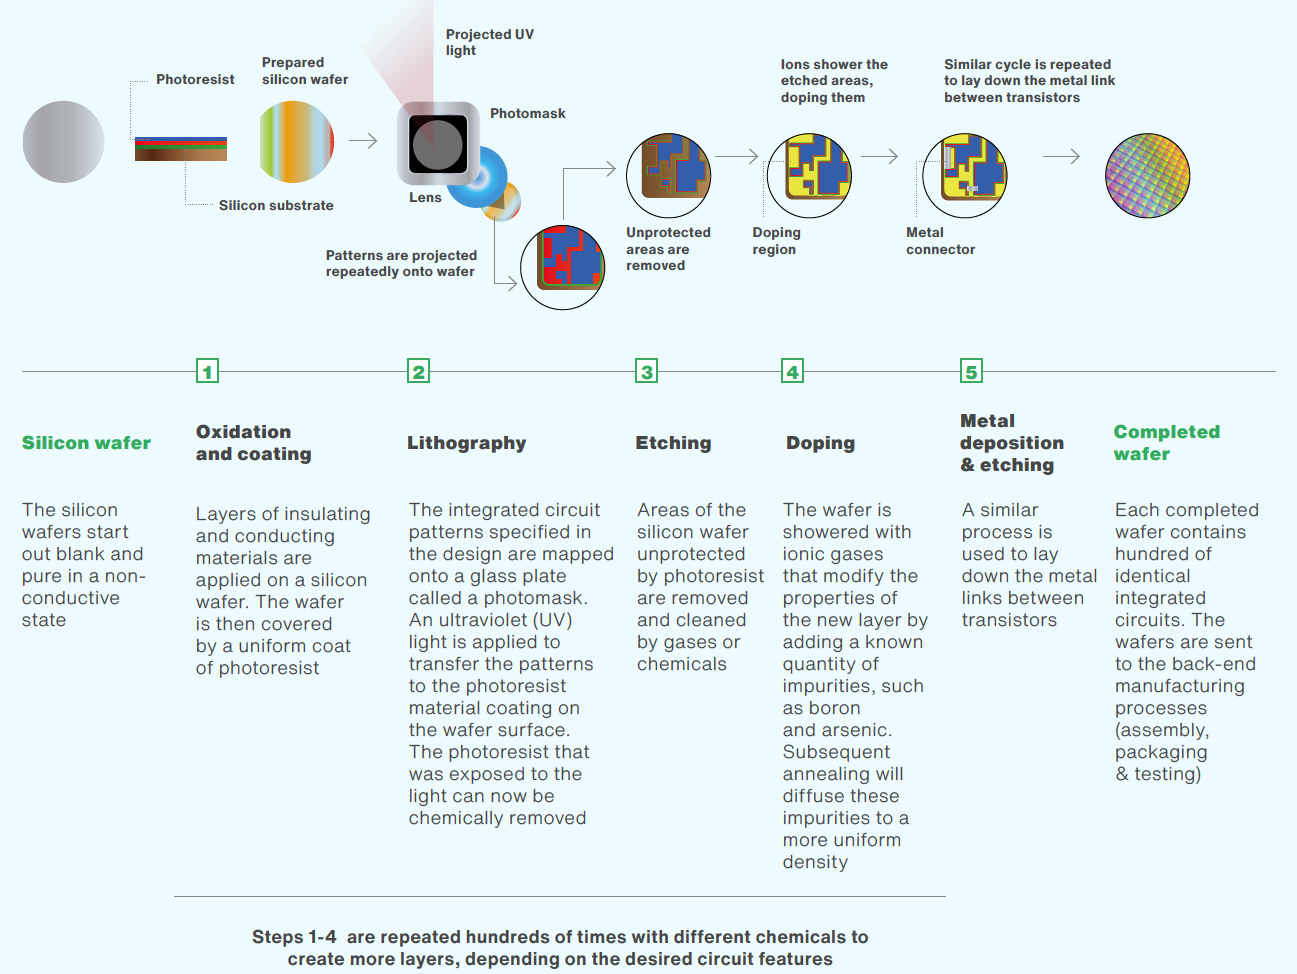
\includegraphics[width=\linewidth]{report/figures/fig_1.2_wafer_manufacturing_process.png}
    \captionsetup{justification=raggedright,singlelinecheck=false}
    \caption*{\footnotesize \textit{Note}. This figure visualizes one pass through the front-end wafer fabrication loop. After a mirror-flat silicon wafer is prepared, the factory repeats a sequence to build each layer: grow or deposit thin films (oxidation and coating), project the circuit image via lithography, remove the uncovered material via etching, introduce controlled impurities via doping, and form metal interconnects via deposition and etching. These steps are executed and measured hundreds of times to create a finished wafer, which then moves to assembly, test, and packaging. Adapted from BCG and SIA, "Strengthening the Global Semiconductor Supply Chain," Exhibit 6 (2021) \parencite{varas_strengthening_2021}.}
\end{figure}

After lithography leaves a patterned photoresist stencil, etching removes the exposed material, transferring the pattern to the underlying film \parencite{van_zant_microchip_2014}. Fabs use two families of processes. Wet etch uses liquid chemistries to dissolve the target layer, while dry (plasma) etch creates a low-pressure plasma whose reactive species and ions remove material from the surface \parencite{coburn_plasma_1979, nishi_handbook_2007}. For the smallest features, tools favor anisotropic plasma etch because it produces straight sidewalls and tight control of the printed line width \parencite{sze_physics_2007}. Two ideas matter throughout: selectivity, meaning the process removes the intended film much faster than the mask or stop layer, and uniformity, meaning the same result is achieved across the full 300~mm wafer, even when feature density varies \parencite{van_zant_microchip_2014,may_fundamentals_2006}. Etch tools use endpoint detection, optical signals, or carefully timed over-etch to stop consistently and then feed those measurements back into recipes to keep profiles in spec during long runs \parencite{may_fundamentals_2006,irds_factory_integration_technical_working_group_international_2023}. For the most delicate layers, fabs also use atomic layer etching (ALE) to remove material cycle-by-cycle with atomic-scale precision and minimal sidewall damage \parencite{kanarik_atomic_2018}. After the main etch, the resist and polymer residues are stripped, and the wafer is cleaned so the next thin film can be deposited on a pristine surface \parencite{nishi_handbook_2007,van_zant_microchip_2014}.

% =========================
% Figure: Lithography in the Wafer-Fabrication Process
% =========================
\begin{figure}[h]
  \centering
  \caption[\textit{Lithography in the Wafer-Fabrication Process}]
  {\textit{Lithography in the Wafer-Fabrication Process}}
  \label{fig:lithography_process}

  % Graphic
  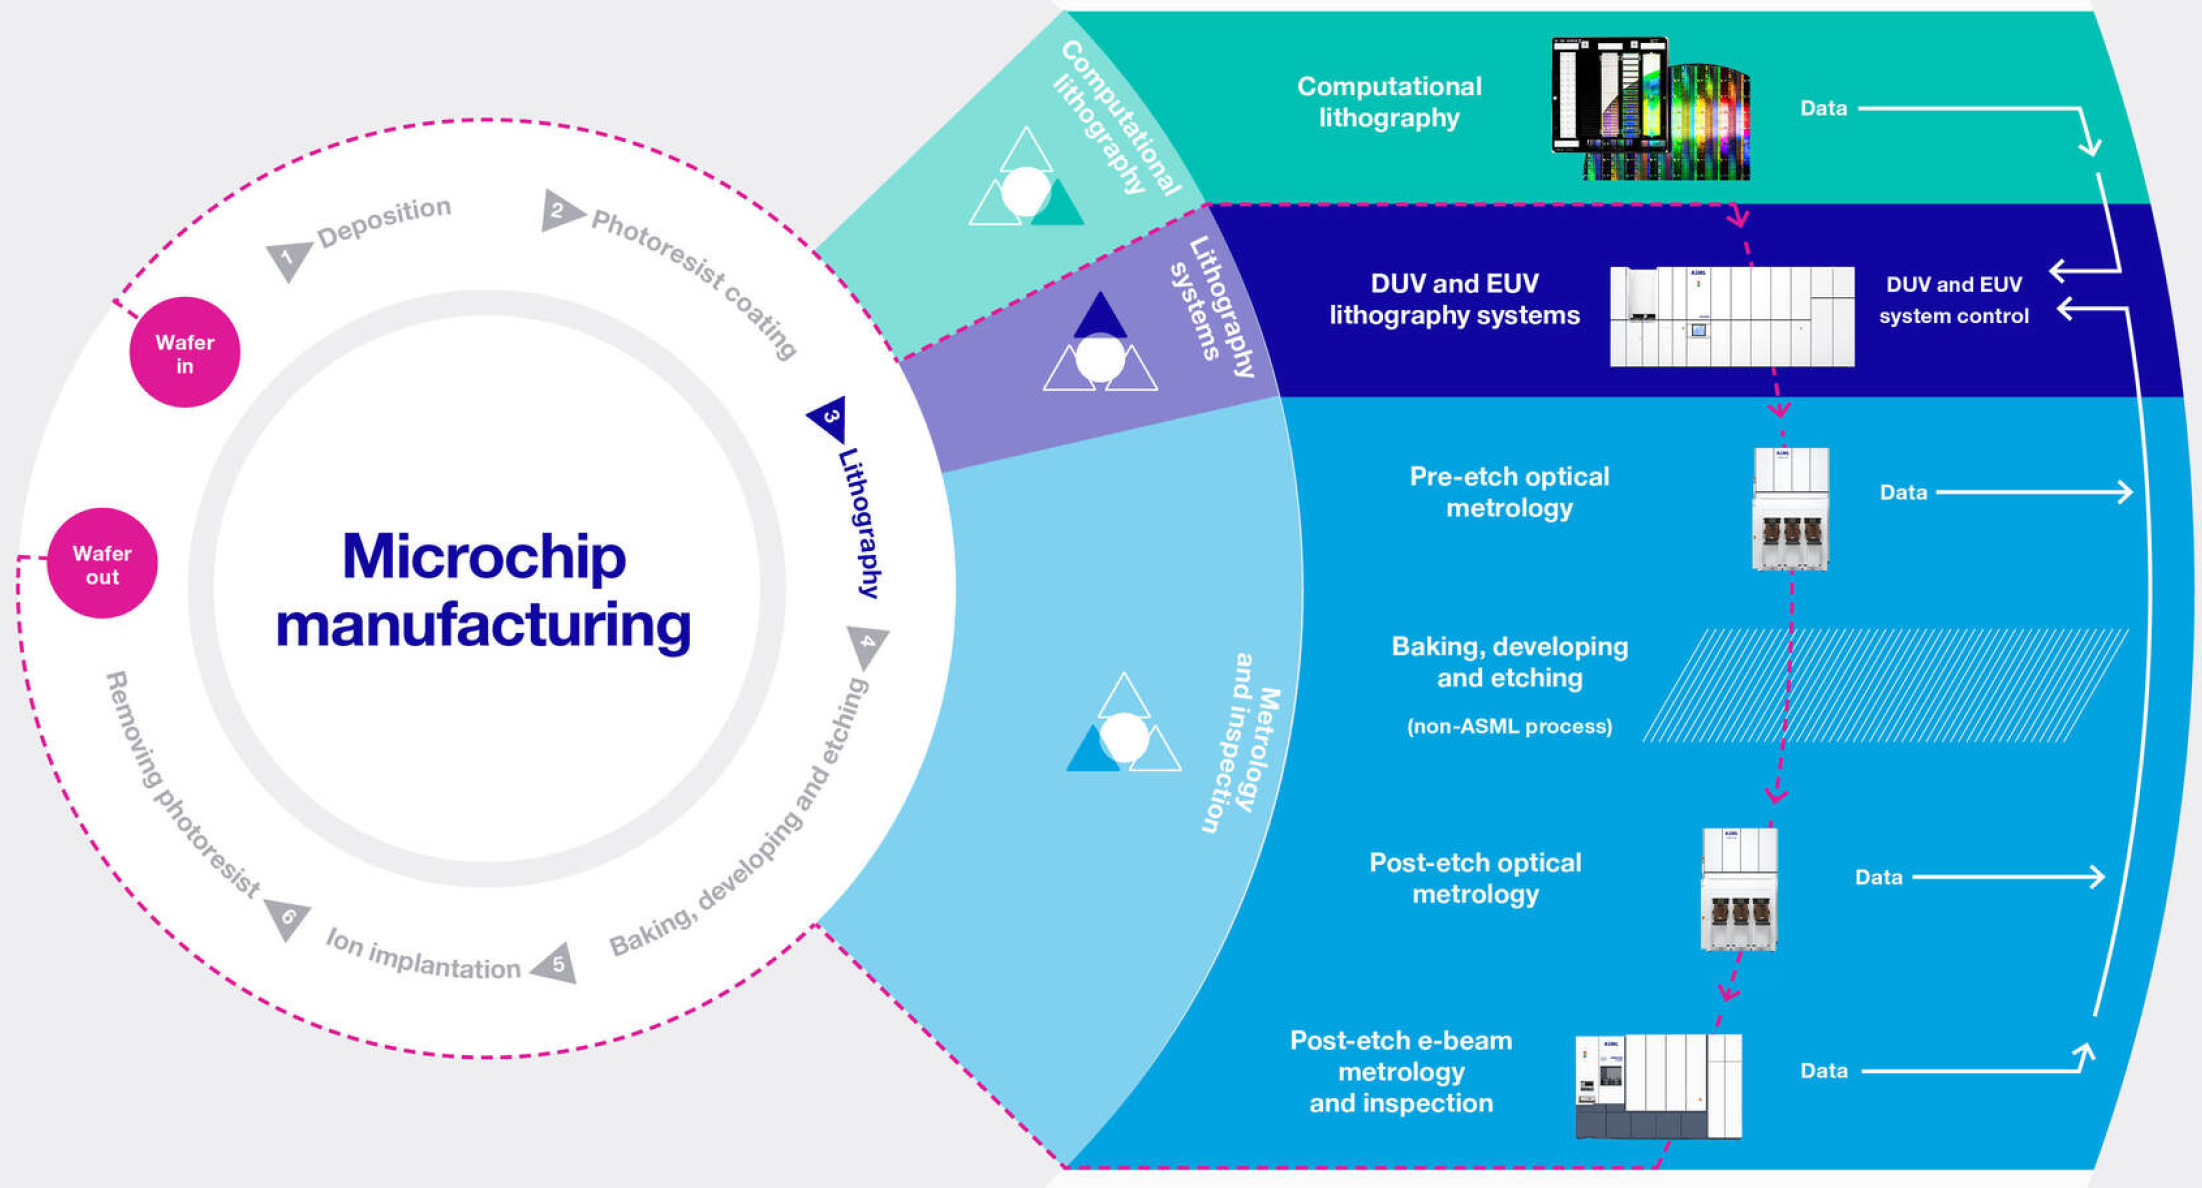
\includegraphics[width=\linewidth]{report/figures/fig_1.3_lithography.png}
    \captionsetup{justification=raggedright,singlelinecheck=false}
    \caption*{\footnotesize \textit{Note}. Lithography is the core patterning that ties the wafer loop together: photoresist coat and bake $\rightarrow$ exposure and development $\rightarrow$ etch $\rightarrow$ pre-/post-etch metrology and inspection, with feedback to hold critical dimension, focus, and overlay to target. Computational lithography and scanner control (deep ultraviolet {DUV} and extreme ultraviolet {EUV}) work in closed loop with optical and e-beam metrology. The cycle repeats across many layers from wafer-in to wafer-out.  Adapted from ASML 2024 Annual Report \parencite{asml_2024_2024}.}
\end{figure}

Some layers require their electrical properties to be modified before the next pattern is built. Fabs introduce dopants, such as boron, phosphorus, or arsenic, into selected regions to make silicon p-type or n-type, enabling transistors to switch and wires to carry current as designed \parencite{sze_physics_2007}. The most common method is ion implantation, in which dopant ions are accelerated in a beam and embedded at a controlled depth in the wafer. The wafer then undergoes a carefully timed thermal anneal to repair crystal damage from the implant and activate the dopants so they sit in the silicon lattice and contribute carriers \parencite{nishi_handbook_2007}. As device dimensions shrink, these steps are run at tightly controlled temperatures and times so that earlier layers do not diffuse or warp, and so the stress and strain engineered into the device are preserved \parencite{sze_physics_2007,irds_factory_integration_technical_working_group_international_2023}.

After the devices are formed, the factory builds the wiring that connects them into working circuits. Think of this as a stack of insulators and metals laid down in many layers. The insulator is patterned first with holes (vias) and grooves (trenches) wherever a connection is needed. Thin foundation films are then added, and the features are filled with metal, most often copper. Tools use a mix of techniques---physical and chemical vapor deposition for the thinnest films, atomic layer deposition for uniform coatings on complex shapes \parencite{puurunen_surface_2005}, and electroplating to quickly fill the larger features \parencite{nishi_handbook_2007,seshan_handbook_2018}. After filling, the surface is planarized by chemical-mechanical polishing (CMP), so the next layer starts flat and in focus for lithography \parencite{van_zant_microchip_2014,may_fundamentals_2006}. This build-fill-polish sequence is repeated many times to form the full interconnect stack. Along the way, inline metrology checks line widths, film thickness, and alignment so electrical resistance and capacitance stay within target, and the design's timing still works as layers add up \parencite{irds_metrology_technical_working_group_international_2023,irds_factory_integration_technical_working_group_international_2023}.

Every few steps, the fab measures what it just made, so the next step starts on target. Tools check critical dimensions---the printed line widths---with specialized electron microscopes (CD-SEM) \parencite{diebold_handbook_2001,irds_metrology_technical_working_group_international_2023}. Film thickness and shape are measured using optical methods, such as scatterometry and ellipsometry. They verify overlay by measuring how well a new layer aligns with marks from the layers below, a capability identified as a cross-cutting need for advanced nodes \parencite{irds_metrology_technical_working_group_international_2023}. Defect inspection scans for particles and pattern errors to find contamination and fix it early \parencite{diebold_handbook_2001}. These data feed statistical process control and small recipe adjustments that nudge tools back into spec or flag maintenance when drift appears \parencite{may_fundamentals_2006,irds_factory_integration_technical_working_group_international_2023}. Because a modern product repeats this loop hundreds to thousands of times, small corrections made early prevent large misses later and help keep yield and schedule on track \parencite{irds_factory_integration_technical_working_group_international_2023}.

Fab cycle time runs several weeks because wafers spend as much time waiting as they do processing \parencite{varas_strengthening_2021}. Lots queue at shared tools, especially lithography scanners, while mask readiness, reticle inspection, and resist track availability link steps that must fire in a precise order \parencite{irds_factory_integration_technical_working_group_international_2023}. Inline measurements can hold a lot while data are reviewed, recipes are tuned, or a short rework is run to bring the line back on target \parencite{may_fundamentals_2006}. The calendar is set by dispatch rules and scheduling, by how well nominally identical tools are matched, and by how quickly the fab responds to drift with maintenance and recalibration \parencite{irds_factory_integration_technical_working_group_international_2023}. Capacity is lumpy because scanners, etchers, and metrology tools are indivisible assets, so a single down tool or a queueing imbalance can stretch cycle time across whole areas of the line \parencite{varas_strengthening_2021}. Factory decisions about workflow, tool matching, and data feedback are reflected directly in the calendar, and small slowdowns repeated across hundreds to over a thousand steps add days or weeks to delivery \parencite{irds_factory_integration_technical_working_group_international_2023}.

The pace of the fab depends on specialized, concentrated semiconductor manufacturing equipment (SME) and critical materials that are often hard to substitute. Lithography scanners, resist tracks, metrology tools, and etch and deposition chambers come from a short list of global suppliers; readiness of photomasks and pellicles gates patterning; and photoresists, high-purity gases, and CMP slurries and pads must meet tight specs to keep yield on track \parencite{varas_strengthening_2021,semiconductor_industry_association_2025_2025}. Several of these inputs exhibit high geographic and firm concentration, creating single-point dependencies in the chain \parencite{oecd_measuring_2019}. For example, fluorinated process gases used in advanced etch are supplied by a handful of firms and may be subject to export controls or industrial incidents. At the same time, advanced resist chemistries and pellicle films have small supplier sets and long qualification times \parencite{kim_potential_2019,varas_strengthening_2021}. Because these inputs touch every wafer and every layer, even small disruptions at this tier can ripple into weeks of delay unless pre-qualified alternates exist \parencite{irds_factory_integration_technical_working_group_international_2023}.

Before wafers leave the front end, the fab runs electrical tests on each die to screen functionality and measure key parameters. Probe cards contact tiny test pads to exercise logic, memory, and interfaces, and the results bin dies by performance and power so later stages can match parts appropriately \parencite{varas_strengthening_2021}. Parametric structures scattered across the wafer also track line widths, resistance, capacitance, and device thresholds, so the line can spot drift and tighten recipes \parencite{irds_factory_integration_technical_working_group_international_2023}. The output of this step is known-good die (KGD)---dies that meet spec well enough to move to packaging and system integration. KGD matters for throughput: catching problems here prevents wasting substrates, attach time, and test capacity downstream, and it helps ATP lines plan for realistic yields and mix.

The front end closes when the wafer's top metal and protective passivation are complete, and the dies have passed wafer sort as known-good die \parencite{irds_factory_integration_technical_working_group_international_2023}. If the package uses flip-chip, the fab may add a thin under-bump metallization and form tiny solder bumps or copper pillars on each die pad while the chips are still on the wafer; these features will make the electrical and mechanical connections to the package substrate \parencite{nishi_handbook_2007}. The wafer is then thinned to its final thickness and singulated---that is, cut into individual chips--- so good dies can be picked, packed, and shipped with their test data to the assembly, test, and packaging (ATP) line \parencite{nishi_handbook_2007, varas_strengthening_2021}. Some flows add package features at the wafer scale before the cut. A common example is a redistribution layer (RDL)---very thin metal traces built on top of the die to move tiny on-chip pads outward so they match the larger pads of a package substrate \parencite{ieee_electronics_packaging_society_heterogeneous_2024,garrou_handbook_2008}. In fan-out packaging, the bare die is first embedded in a mold material, and then RDL is built on the molded surface, creating a compact package with more connections than the die footprint alone would allow \parencite{garrou_handbook_2008}. Whether these steps happen at the fab or the ATP site, the shift is the same: production moves from patterning silicon to joining, protecting, and testing chips so they can be mounted on boards and used in systems.

The third and final production phase is assembly, test, and packaging (ATP). This stage moves beyond the fab and into the processes that join, protect, and verify chips for use on boards and in systems. Beyond traditional wire-bond and flip-chip packages, today's ATP often integrates multiple chips into a single module: side-by-side on a thin silicon interposer (2.5D) or stacked vertically with through-silicon vias (TSVs) or hybrid bonding (3D) to reduce interconnect length, increase bandwidth, and lower power consumption \parencite{garrou_handbook_2008}. A clear example is high-bandwidth memory (HBM), which stacks several DRAM layers on a base logic die and connects them with dense vertical wiring to feed GPUs and AI accelerators \parencite{jedec_jesd238_hbm3_2022}. These structures introduce mechanical and thermal challenges---heat removal in thick stacks, warpage control as materials expand differently, and clean power and clock delivery through tiny bumps or copper-to-copper bonds---so packaging choices are co-designed with die, interposer, and redistribution-layer layouts \parencite{ieee_electronics_packaging_society_heterogeneous_2024}. They also raise the bar for package-level reliability: packages see temperature cycling, humidity, vibration, and mechanical shock, so programs run burn-in and environmental screens and follow JEDEC/MIL-class test flows to qualify materials, joints, and assemblies before ship \parencite{bailey_reliability_2025,department_of_defense_test_2025}. The payoff is large, more performance per watt in a smaller footprint, but it depends on close coordination between die design, interposer/RDL layout, materials selection, and test strategy, because in advanced packages the boundary between "chip" and "package" is now a design choice rather than a hard line \parencite{ieee_electronics_packaging_society_heterogeneous_2024}.

The preceding sections traced the full production arc. Design produces verified layouts and mask data. The wafer passes through materials and crystal growth, then into the fab, where layers are built by repeating film deposition, lithography, etch, clean, doping/anneal, interconnect formation, and constant measurement and control. Factory integration, scheduling, tool matching, mask readiness, and feedback turn physics and process into a calendar. Finally, assembly, test, and packaging (ATP) joins, protects, and qualifies dies, and advanced packaging now places multiple chips side-by-side or in vertical stacks to meet bandwidth and power goals \parencite{varas_strengthening_2021,irds_factory_integration_technical_working_group_international_2023,ieee_electronics_packaging_society_heterogeneous_2024}. The next section uses this structure to motivate the network mapping that follows, and to show why some of the most consequential dependencies in the DoD-relevant supply chain live not only in final-assembly contractors, but also in the tool, materials, and packaging tiers that pace readiness and delivery \parencite{oecd_measuring_2019,khan_semiconductor_2021}.

% ===========Section 1.4 The Semiconductor Supply Chain======================
\section{The Semiconductor Supply Chain}
\label{sec:sc-network}

This section widens the aperture from unit processes to the system that moves designs, tools, materials, and knowledge across borders. Where the manufacturing section traced choreography inside fabs and assembly, test, and packaging (ATP), the supply chain lens shows how those steps are distributed globally and coordinated through logistics, standards, and contracts. At this level, the semiconductor supply chain is complex, global, interdependent, and opaque, with critical work spread across regions and stitched together by cross-border flows that no single firm or country controls \parencite{thadani_mapping_2023,oecd_measuring_2019}. What moves are not only wafers and parts but enabling artifacts---process design kits (PDKs), mask data, electronic design automation (EDA) toolchains and core IP, test programs, and process recipes---that gate whether production can start, proceed, or ship \parencite{neisser_international_2021, palma_growing_2022}. This section describes the multi-tier network and how it operates in practice, distinguishing physical shipments from the enabling links so that the real sources of constraint and leverage are visible.

A small set of supply-chain and network terms clarifies the discussion that follows. A node is an actor or site that performs, moves, or enables a step---usually a firm---and, when location matters for capability or risk, a specific fab, assembly, test, and packaging (ATP) facility \parencite{newman_networks_2010}. An edge records a supply relationship between two nodes, with the direction running from the supplier to the recipient. Edges can carry physical goods or enablers, such as process design kits (PDKs), mask data, test programs, and metrology recipes. Weights summarize the strength or risk of a link. They can represent volume or expenditure, lead time, uniqueness or substitutability, and the cost and time to re-qualify if the supplier changes \parencite{borgatti_social_2009}. Tiers count how many steps away a node sits from a focal product: Tier-1 is the direct supplier, Tier-2 supplies Tier-1, and the pattern continues outward \parencite{jackson_social_2008, newman_networks_2010}. With those terms in mind, consider a slice you just saw in manufacturing: a fab is a node that depends on photoresist deliveries from a chemical plant (a material edge) and on mask data and a PDK from the design and foundry technology teams (enabling edges) \parencite{khan_semiconductor_2021}. The direction runs into the fab, and the enabling edges gate the step (no mask data), resulting in no exposure. At the same time, weights capture the amount of resist consumed and the difficulty of switching to a different resist or PDK without re-qualification.

No single country or company covers the entire semiconductor stack, and the division of labor is not accidental \parencite{palma_growing_2022}. The United States anchors electronic design automation (EDA), core intellectual property (IP), and much of the highest-value chip design; Europe leads in optics-heavy manufacturing equipment and specialized materials; Taiwan and South Korea operate the most advanced wafer fabrication; Japan supplies wafers, photoresists, precision chemicals, and key gases; and China and Southeast Asia host a dense assembly, test, and packaging capacity (ATP) while expanding in multiple steps \parencite{semiconductor_industry_association_2025_2025, kim_potential_2019}. These roles reflect accumulated know-how, supplier ecosystems, and policy histories that are difficult to replicate quickly. The result is a production system linked by cross-border flows of equipment, precursors, reticles and pellicles, advanced organic substrates, and metrology know-how \parencite{thadani_mapping_2023}. Because capabilities are distributed, national self-sufficiency is not presently feasible for leading-edge nodes, and attempted reshoring triggers long sequences of supplier development and re-qualification \parencite{palma_growing_2022}.

Two business models organize the way chips are made and help explain why the supply chain looks the way it does. Integrated device manufacturers (IDMs) keep design, wafer fabrication, and often packaging under one roof, yet they still depend on external equipment and materials sourced globally \parencite{oecd_measuring_2019}. The alternative unbundles the stack into "fabless" design firms, merchant foundries, and outsourced assembly and testing (OSAT), a division driven by extreme capital intensity in fabs, scale economies, and steep learning curves that reward specialization and high utilization \parencite{sturgeon_global_2010,oecd_measuring_2019}. This modular model moves more enabling artifacts across firm boundaries, since process design kits (PDKs), mask data, design IP, and test assets must align across companies and borders for each run to proceed \parencite{palma_growing_2022}. Even IDMs often rely on contract packaging or specialized processes outside of their walls, so neither model eliminates the dependence between regions \parencite{khan_semiconductor_2021}. In network terms, foundries and OSATs sit on many of the paths between designers and critical inputs, thereby concentrating leverage and raising the premium on visibility into sub-tiers.

% =========================
% Figure: The Global Journey of a Chip
% =========================
\begin{figure}[tbp]
  \centering
  \caption[\textit{The Global Journey of a Chip}]
  {\textit{The Global Journey of a Chip}}
  \label{fig:global_journey}

  % Graphic
  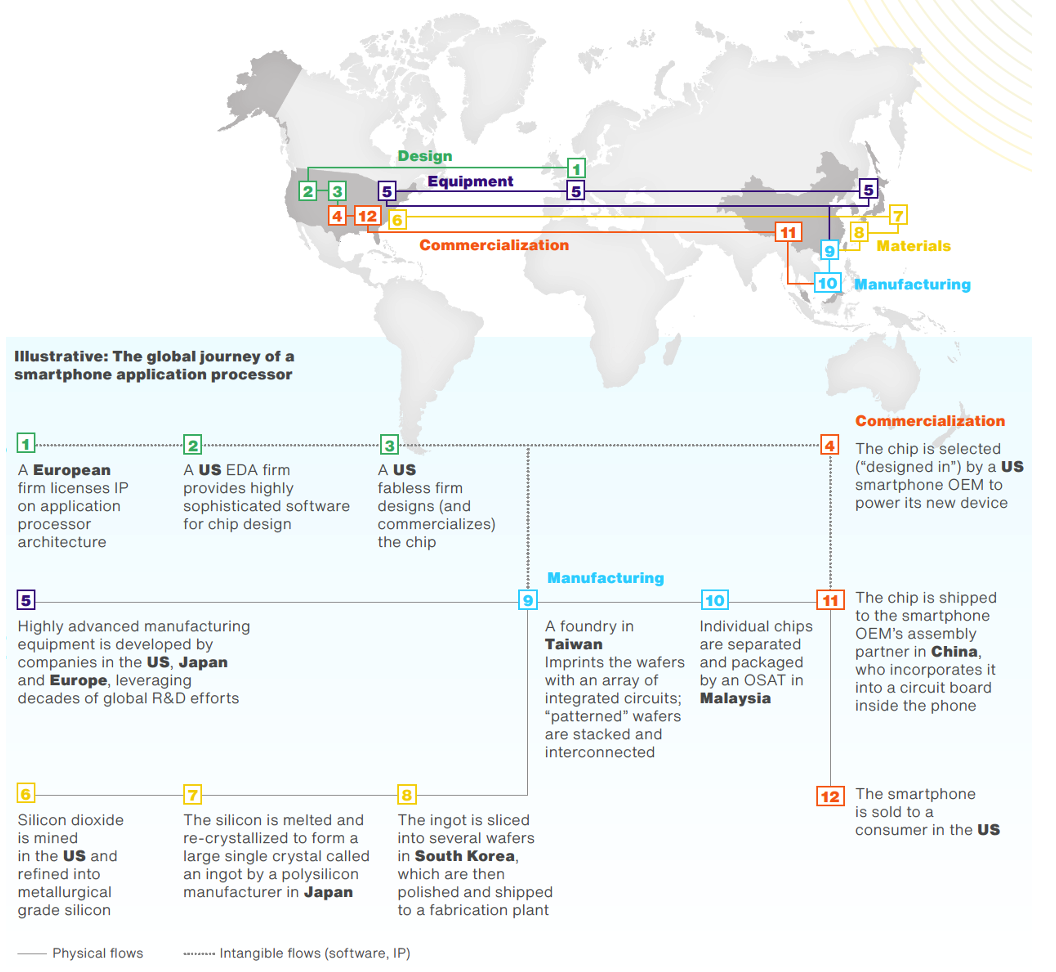
\includegraphics[width=\linewidth]{report/figures/fig_1.4_global_journey.png}
    \captionsetup{justification=raggedright,singlelinecheck=false}
    \caption*{\footnotesize \textit{Note}. Semiconductor production is inherently transnational: a typical device traverses the United States, Europe, Taiwan, South Korea, Japan, and China/Southeast Asia as design/IP and equipment (dashed) and materials and wafers (solid) move from concept to packaged part. In 2019, each of these regions accounted for at least 8\% of global value added, underscoring the structural interdependence. Adapted from BCG and SIA, "Strengthening the Global Semiconductor Supply Chain," Exhibit 6 (2021) \parencite{varas_strengthening_2021}. }
\end{figure}

A single commercial chip is a cross-border project: its viability depends on synchronized hand-offs of tools, materials, and enabling artifacts across multiple regions. Architecture and IP blocks are composed using electronic design automation (EDA) in the United States and Europe, and mask data and process design kits (PDKs) are then shipped to a wafer fab in Taiwan or South Korea \parencite{varas_strengthening_2021, semiconductor_industry_association_2025_2025}. Lithography in that fab runs on extreme ultraviolet (EUV) scanners from the Netherlands with precision optics from Germany, while photoresists and fluorinated process gases arrive from Japanese chemical clusters \parencite{asml_2024_2024, thadani_mapping_2023}. After front-end processing, the wafers are shipped to outsourced assembly, test and packaging (ATP) providers in Malaysia, Vietnam, or China, where test programs and advanced organic substrates complete the package \parencite{thadani_mapping_2023}. Figure~\ref{fig:global_journey} maps this journey and shows that a single chip typically touches all six major semiconductor regions-the United States, Europe, Taiwan, South Korea, Japan, and China/Southeast Asia \parencite{varas_strengthening_2021}. The journey thus spans multiple borders and depends on distinct regional ecosystems that no single firm or country controls.

The cross-region dependence is clearest in the market for semiconductor manufacturing equipment and the consumables used with it. No fab sources an entire line from one country. Lithography, etch, deposition, and metrology tools are sold, installed, and serviced across regions, with process-control software, spares, and field support moving with them \parencite{thadani_mapping_2023}. High-spec materials---photoresists, advanced precursors, and ultra-clean gases---follow similar routes and require re-qualification when sources change. Figure~\ref{fig:sme-sales} summarizes these exchanges: sellers and purchasers in each region trade across tool categories, so that a capacity addition in one country still depends on imported systems and inputs. These patterns suggest that policy shocks and export controls tend to rewire flows rather than eliminate reliance, reinforcing the structural nature of interdependence.

% =========================
% Figure: Semiconductor Manufacturing Equipment Sales
% =========================
\begin{figure}[h]
  \centering
  \caption[\textit{Semiconductor Manufacturing Equipment Sales}]
  {\textit{Semiconductor Manufacturing Equipment Sales and Purchases
  (2021, in billions)}}
  \label{fig:sme-sales}

  % Graphic
  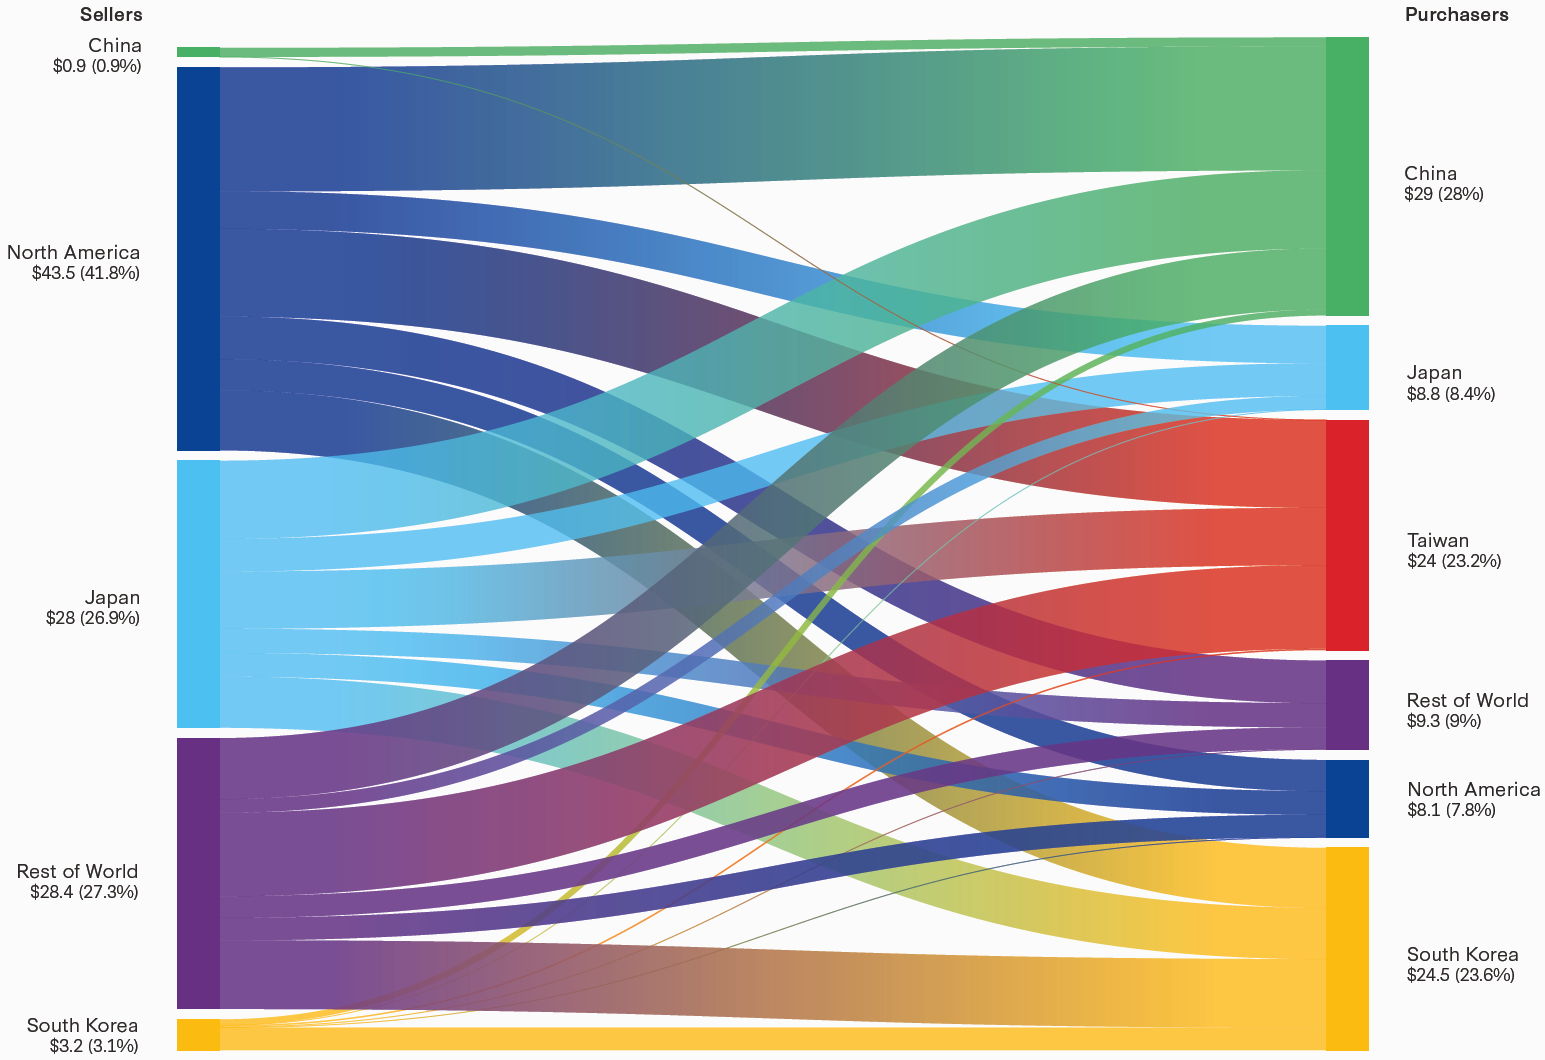
\includegraphics[width=\linewidth]{report/figures/fig_1.5_sme_sales.png}
    \captionsetup{justification=raggedright,singlelinecheck=false}
    \caption*{\footnotesize \textit{Note}. This diagram visualizes source-destination flows by region for semiconductor manufacturing equipment, with sellers on the left and purchasers on the right. Bandwidth scales with the value of shipments, making the cross-border nature of tool procurement visible. \textit{Adapted from}: Thadani and Allen, \textit{Mapping the Semiconductor Supply Chain: The Critical Role of the Indo-Pacific Region} (CSIS, May 2023) \parencite{thadani_mapping_2023}.}
\end{figure}

Narrow capabilities create real chokepoints in which substitution is difficult, and requalification is slow. Extreme ultraviolet (EUV) optics and pellicles operate to nanometer tolerances, and if they are not available or out of spec, exposures stop production and require extensive retuning and reliability checks \parencite{asml_2024_2024,neisser_international_2021}. Photoresists and their precursors are co-tuned to scanners and recipes, so a source change propagates through process windows \parencite{irds_lithography_technical_working_group_international_2023}. Fluorinated process gases must meet ultra-high-purity thresholds and stable impurity profiles, and qualification of a new stream involves recalibration and yield learning that few manufacturing facilities accept mid-run \parencite{irds_lithography_technical_working_group_international_2023}. In the back end, advanced organic substrates for high-density packages demand fine lines, controlled coefficients of thermal expansion, and low loss, and capacity is concentrated in facilities that are difficult to replicate quickly. Metrology toolchains, overlay, critical-dimension, and defect inspection are woven into process control, and swapping them resets baselines and model parameters in multiple steps \parencite{irds_metrology_technical_working_group_international_2023}. Because only a handful of providers can meet these specifications at scale with the required contamination control, shocks to these inputs are translated into schedule slips and yield risk. That concentration gives their suppliers structural leverage over the system.

A system this complex, global, and interdependent is also hard to see beyond the first tier. Opacity in this system is not an accident; it is built into how firms transact. Non-disclosure agreements and foundry confidentiality keep sub-tier relationships private, and multi-party subcontracting hides which provider delivers the enabling inputs that make a Tier-1 purchase order executable. Public reports aggregate suppliers by category, and contracts often bar onward disclosure, so reticles, pellicles, photoresists, fluorinated gases, process design kits (PDKs), and test programs rarely appear alongside the prime vendor on any document. Tool vendors layer in service contracts and remote diagnostics, creating additional dependencies that are material to operations but are not visible in standard spend data. The result is a visible Tier-1 and a largely hidden enabling stack, which complicates risk assessment and response planning. Policy reviews have called for multi-tier mapping and deeper traceability to close this gap, and emphasize linking design-time artifacts and process knowledge to access, rather than listing only prime suppliers \parencite{TheWhiteHouse2021,chips_research_development_office_vision_2023, us_department_of_commerce_defense_2009, ch5_dod2022_supplychains}.

Together, the picture that emerges is a world-spanning production system that is complex, interdependent, opaque, and hard to substitute. No single country or company covers the full stack, and the work is deliberately specialized by region, with cross-border hand-offs that move both physical goods and enabling artifacts such as process design kits, mask data, and test programs. Tooling and materials follow the same pattern, which means that a capacity addition in one country still depends on imported lithography, etch, deposition, and metrology systems, as well as their service ecosystems. Narrow capabilities---EUV optics and pellicles, advanced resists and precursors, fluorinated gases, high-density substrates, and integrated metrology---create chokepoints that few providers can meet at spec and at scale. These features make the system efficient and innovative, yet they also concentrate leverage and turn distant disruptions into local schedule and yield risk.

The opacity compounds this risk. Tier-1 purchase orders and public reports rarely reveal the enabling sub-tiers that make delivery possible, because non-disclosure agreements, foundry confidentiality, and subcontracting keep those relationships out of view \parencite{oecd_measuring_2019}. As a result, many of the most consequential dependencies on specific reticles and pellicles, chemistries, gases, or service entitlements are material to operations but invisible in standard datasets. Recent policy reviews call for multi-tier mapping and deeper traceability that link design-time artifacts and process knowledge to access, rather than just listing prime vendors. The next section introduces a taxonomy of vulnerabilities that follow from this structure and explores how they can cascade into strategic risks for the DoD.


% ===========Section 1.5 Vulnerabilities: Continuity vs. Integrity==========
\section{Vulnerabilities: Continuity vs.\ Integrity}
\label{sec:risk-classes}

Two vulnerability classes are distinguished: continuity risk, which reduces or delays output, and integrity risk, which degrades trust in what ships. Continuity is the risk that parts do not arrive when needed, because chipmaking runs in long, tightly sequenced batches that must be re-verified after any interruption; small stoppages quickly turn into long schedule slips. Integrity speaks to the assurance of components and toolchains whose provenance and behavior must be trusted at the moment of need. This framework aligns with the defense and standards literature, which treats microelectronics as a mission-critical infrastructure and separates assured access to parts from confidence that the parts are free of counterfeits, defects, or malicious insertions \parencite{defense_science_board_report_2005,kahn_semiconductors_2023}. It also reflects recent policy usage, in which the Department of Defense and advisory bodies call for illumination of supply networks to precisely manage both availability and trust \parencite{ch5_dod2022_supplychains,defense_science_board_report_2005}. In what follows, this taxonomy organizes historical evidence of how disruptions arise and how their effects cascade in practice, reserving mitigation choices for later sections \parencite{wasser_when_2022}.

By "continuity," this report means the risk that an adversary, a policy shock, or a natural shock interrupts the flow of chips that U.S. forces consume every day, much as they consume munitions, spare parts, and fuel. The semiconductor chain is long, specialized, and cross-border. Many of its most vulnerable points sit deep below tier 1, where single firms supply lithography subsystems, mask and pellicle blanks, photoresists and fluorinated gases, advanced organic substrates, or critical packaging and test capacity \parencite{varas_strengthening_2021,thadani_mapping_2023}. An adversary need not crater a flagship fab to matter. Disrupting a key chemical plant, a reticle supplier, a substrate line, or a handful of logistics and software service nodes can deny or delay output that the Department of Defense ultimately relies on for aircraft, missiles, radios, night-vision devices, and command-and-control systems \parencite{wasser_when_2022,usdoe_office_of_energy_efficiency_and_renewable_energy_eere_semiconductor_2022}. Because these tiers are tightly coupled across regions, a disruption at one node easily cascades across the entire network. The effect is a broader schedule shock that shows up in program timelines and operational availability.

Continuity risks arise from many directions, but they all do the same thing: they interrupt the global flow of chips and trigger a cascade that manifests far from the initial trigger. The COVID-19 pandemic led to shutdowns of major Asian semiconductor fabs and logistics bottlenecks, triggering a worldwide chip shortage that rippled from consumer electronics to automotives, and served as a wake-up call that overreliance on foreign nodes can become a mission-critical problem for defense programs as well \parencite{wasser_when_2022,department_of_defense_assured_2025,usdoe_office_of_energy_efficiency_and_renewable_energy_eere_semiconductor_2022}. Natural hazards and industrial accidents have had the same effect. Japan's 2011 Tohoku earthquake/tsunami shut down a critical microcontroller fab for three months, severely impacting global electronics supply \parencite{matsuo_implications_2015}. In 2021, an electrical fault at Renesas Electronics' Naka plant in northeast Japan caused a fire that shut down a 300mm wafer line producing automotive microcontrollers, forcing Toyota, Nissan, and Honda to scramble for alternative supply; with Renesas holding roughly 30\% of the global automotive MCU market, the disruption rippled across the industry for months \parencite{reuters_japanese_2021}. More recently, a 7.4-magnitude earthquake in April 2024 forced Taiwanese chipmaker TSMC to halt production for safety inspections---a short-term disruption that analysts warned could tighten global semiconductor supply and raise prices downstream \parencite{usgs_hualien_2024,reuters_tsmc_earthquake_2024}. These events highlight extreme continuity risks: a single catastrophe in a semiconductor hub can delay production and delivery of chips worldwide.

Geopolitical export controls have exposed supply fragility. In 2019, Japan abruptly tightened export curbs on three specialty chemical materials vital for chip fabrication (photoresists, hydrogen fluoride, etc.) in a dispute with South Korea, threatening to disrupt the global tech supply chain since Japan produced $\sim$70\% of those inputs. This incident forced the Korean chip giants Samsung and SK Hynix to scramble to secure alternative suppliers. It highlighted how diplomatic conflicts can jeopardize the continuity of supply for business-critical microelectronics \parencite{yamazaki_japans_2019, kim_potential_2019, usitc_japan_korea_2020}. Similarly, events like China's rare-earth metals ban foreshadow how sanctions and strategic embargoes can cut off essential chip materials, putting production at risk \parencite{mak_chips-for-rare-earths_2025, csis_china_rare_earth_2025}.

Not all continuity risks are physical. Adversaries that want to slow, complicate, or deny U.S. access to specific components can exploit the network's digital and organizational seams---malware introduced through plant IT or third-party service channels, disruptions to tool-vendor remote support, attacks on freight forwarders and customs brokers, or manipulation of licensing and certification chokepoints---to knock upstream nodes offline and sow cascading delays \parencite{ch5_dod2022_supplychains,wasser_when_2022}. The 2018 malware incident at TSMC, the world's largest foundry, which shut multiple bays and led to missed shipments, illustrates how a single piece of malicious code can trigger plant-wide stoppages and propagate schedule slip across customers, even without a fire or an earthquake \parencite{tsmc_tsmc_2018}. For an actor intent on imposing costs on U.S. programs, this is a playbook: there is no need to touch a Pentagon facility at all; hitting a commercial wafer fab, a materials supplier, or a logistics bridge can achieve the same effect quickly and with plausible deniability. The common thread is simple and central to the Department of Defense: whether the trigger is a pandemic, an earthquake, an export rule, a gas shortage, or malware, nudging a few critical or deep sub-tier nodes off-rhythm produces a global cascade of supply disruption that ultimately erodes the delivery of U.S. military critical supplies.

A final structural point explains why these shocks become calendar math and persist. Much of the chain is surge-limited: leading-edge lithography and etch tools are built by a handful of vendors with long lead times; the optics, resists, and other front-end consumables that feed them are concentrated in a few firms; and advanced substrates and major OSAT lines are booked years ahead \parencite{thadani_mapping_2023}. Water and power are not interchangeable inputs---droughts and grid failures can idle whole campuses, with no easy substitute \parencite{lepawsky_climate_2024}. And because this is a largely private, global supply base, U.S. priority-rating tools have limited reach abroad. Defense programs cannot compel foreign firms or tool vendors to reconfigure capacity on demand \parencite{ch5_dod2022_supplychains,department_of_defense_assured_2025}. The practical upshot is that small nudges at a few narrow points can produce long-lived global cascades---even when the initial trigger is brief or far away \parencite{usdoe_office_of_energy_efficiency_and_renewable_energy_eere_semiconductor_2022}.

If continuity is whether a part shows up, integrity is whether the part that shows up can be trusted to do exactly what it is supposed to do when the pressure is highest. Integrity failures fall into two broad categories: straightforward substitution (the item is not what it claims to be) and malicious modification, in which something real has been altered so that it behaves normally until it quietly fails or misdirects a system at the worst moment. In a military force that relies on digital sensors, networks, and guided weapons, such failures manifest as unexplained glitches, degraded performance, or silent misfires at the wrong moment. They are possible because the defense chip supply runs through long, international chains of parents, affiliates, service providers, and subcontractors, with design know-how and update rights spread across many hands and jurisdictions. The result is a level of complexity and opacity that can be exploited by criminals and, in the worst case, by states' leverage over sub-tier suppliers. These risks are not hypothetical: national reviews have documented counterfeit penetration and warned about hardware-level tampering in defense-relevant electronics, and they treat integrity alongside availability as a core readiness problem \parencite{TheWhiteHouse2021,khan_semiconductor_2021,national_science_and_technology_council_national_2024}.

The clearest evidence that integrity risk is real is the public record on counterfeit penetration of U.S. defense programs \parencite{united_states_senate_committee_on_armed_services_senate_2012}. The Senate Armed Services Committee's 2012 inquiry documented large numbers of suspect and relabeled parts moving from overseas e-waste streams, through broker chains, and into flight displays, collision-avoidance computers, submarine imaging systems, and Army vehicle electronics \parencite{united_states_senate_committee_on_armed_services_senate_2012}. GAO then conducted its own test purchases and found that all 16 parts purchased from internet brokers were counterfeit. \parencite{U.S.GovernmentAccountabilityOffice2012}. A subsequent review identified ongoing weaknesses in reporting and supplier vetting, indicating that the pathway for substitution has not been closed \parencite{U.S.GovernmentAccountabilityOffice2016}. None of this required exotic tradecraft. It exploited long sustainment tails that push programs to secondary markets, thin visibility below the first tier, and paperwork-heavy acceptance processes that check documents rather than provenance. In the field, these parts do not always fail with a single dramatic event. They more often manifest as intermittent faults, early-life failures, and unexpected downtime that erode confidence and availability just when systems are needed most \parencite{TheWhiteHouse2021,guin_counterfeit_2014}. That is why national reviews now treat counterfeit risk as a standing condition of the market and place integrity alongside availability as a core readiness constraint \parencite{TheWhiteHouse2021,ch5_dod2022_supplychains}.

The second form of integrity risk is malicious modification. A genuine component can be built or programmed to include a hidden behavior that triggers under certain conditions, so it appears to work until it quietly fails or misdirects a system \parencite{kahn_semiconductors_2023}. That change can be introduced in design files, in build and test tools, or when firmware and configuration data are loaded late in production. It is hard to detect because normal qualification checks demonstrate that a unit meets performance requirements; they do not demonstrate the absence of a covert feature, and small manipulations can be hidden within normal manufacturing variation \parencite{semiconductor_equipment_and_materials_international_heterogeneous_2021}. Public guidance to defense programs now treats hardware Trojans and toolchain tampering as credible threats and calls for stronger assurance around design, build, and programming steps \parencite{kahn_semiconductors_2023,tehranipoor_hardware_trojan_2010}. The risk is amplified by reuse. The same cores, software, and production tools tend to appear across multiple systems, so a single compromised block or build environment can propagate to programs before anyone is aware. For these reasons, national reviews place hardware-level tampering alongside counterfeits as a core readiness concern, not a niche technical issue \parencite{TheWhiteHouse2021}.

To make the stakes concrete, consider a brief hypothetical scenario. In the first week of a Taiwan crisis, a preplanned strike package assumes thousands of precision weapons will hit on schedule. Months earlier, a state-influenced sub-tier packaging contractor introduced a minor change to the configuration code of a guidance chip used across a family of GPS-aided bombs. The parts met spec, passed acceptance tests, and were placed in stock. In combat, a particular timing pattern causes the added logic to corrupt the navigation update, pushing some weapons off target by tens of meters. Crews see a handful of odd misses and chalk them up to routine interference. Only after a pattern emerges, after sorties and munitions have been spent, does the compromise become clear.

This section has identified two ways in which a chip-dependent force can be affected. Continuity failures slow or stop the flow of parts. Integrity failures deliver parts that cannot be trusted when they matter. Neither risk is hypothetical. The public record already shows both patterns in defense-relevant electronics. Senate and GAO investigations documented substitution and counterfeits moving through broker chains into flight displays, navigation and imaging modules, and vehicle electronics \parencite{united_states_senate_committee_on_armed_services_senate_2012,U.S.GovernmentAccountabilityOffice2012}. National supply-chain reviews describe how global specialization, long sustainment tails, and cross-border ownership and service rights create seams that criminals and states can exploit, including through sub-tier leverage and toolchain access \parencite{khan_semiconductor_2021,national_science_and_technology_council_national_2024}. On the flow side, recent crises and incidents have shown how shocks at a single node---from export holds to plant outages---cascade across tiers and supply networks.

What makes these vulnerabilities durable is the network's structure. Defense-relevant chips are born of long, opaque chains that stitch together designers, IP holders, foundries, packaging houses, and remote service providers working under different legal regimes. The same features that make the sector fast and efficient---deep reuse of cores and tools, remote update paths, international joint ventures, and majority stakes in sub-tier suppliers---can also become attack surfaces. An adversary need not reach a prime contractor or a U.S. fab. Pressure on a lower-tier owner, a mask or packaging partner, or a service channel can buy visibility or control, or it can inject something that passes qualification but fails under stress. Conversely, a single export decision or service cutoff can deny flow to multiple programs simultaneously. For the Department of Defense, the practical takeaway is clear. In a global chip system, mission risk arrives in two forms: denied supply and corrupted trust, and both are amplified by the same complexity and opacity that power the industry.

% ================Section 1.6 The DoD Visibility Problem==============
\section{The DoD Visibility Problem}
\label{sec:visibility-pipeline}

The preceding risk taxonomy establishes what can go wrong; this section describes how the report makes those risks visible. The Department of Defense cannot fix what it cannot see. Sightlines are thin beyond prime vendors, so visibility is built in stages, starting broad and narrowing to the DoD semiconductor subgraph. First, a global, disclosed firm-to-firm network is assembled from commercial financial relationship data (FactSet), and an ensemble of link-prediction models is trained to detect likely hidden ties. The DoD supply chain is then seeded with government contracting data to identify Tier-1 vendors, project their upstream tiers within the disclosed network, extend the network with predicted links (including firms not initially present), and layer shipment observations to mark \emph{observed} exchanges. Finally, the build is pruned to semiconductor-relevant nodes and deepened upstream across material and information flows, stitching the results into a decision-grade subgraph. The sequence is \textbf{Disclosed} $\rightarrow$ \textbf{Predicted} $\rightarrow$ \textbf{Observed} because visibility precedes defense. This auditable map anchors the continuity and integrity risk analysis that follows. Model details and evaluation appear in later sections.

The defense-relevant microelectronics ecosystem is modeled as a directed, time-stamped, multi-tier network. Nodes are firms. Edges run from supplier to recipient and include two intertwined layers: \emph{material flows} that move inputs, parts, and services, and \emph{information flows} that move enabling artifacts such as process design kits, mask data, core IP, test programs, firmware, and tool-service entitlements. Each node carries attributes relevant to analysis and policy, including industry role, geography, and ownership and control. This representation converts vendor lists into a routable map, supports tiered views, and reveals how dependencies accumulate and where a disruption could propagate.

The data posture is simple: open or commercially licensed sources only, with every transformation logged so the build is auditable and reproducible. All data are unclassified and, by their nature, available to any adversary of the United States. The value here is integration and rigor, not privileged access. At a high level, the build combines commercial firm-to-firm relationship data, U.S. government contracting records, and public shipment signals, and it enriches nodes with industry, geography, and ownership attributes. Entities are resolved to a stable master, start and end dates are tracked on edges, and point-in-time snapshots are maintained, enabling figures and tables to be regenerated exactly. Each run produces a versioned ledger that records inputs, code revisions, and checks on directionality and coherence. The focus is organizational and facility-level, not individual, and the build adheres to license and disclosure constraints. Detailed schemas and procedures appear in Section~\ref{chap:link-prediction}.

The build begins with a global, firm-to-firm graph assembled from commercial relationship records. Directions are normalized from supplier $\rightarrow$ recipient, entities are reconciled to a single master, and start and end dates are retained with explicit source provenance, along with core attributes such as industry role, geography, support filtering, and tier traversal. This baseline anchors what is known and provides the scaffold for the next two stages. When DoD Tier-1 is later seeded using contracting data, upstream tiers are projected within this disclosed graph before layering predictions and observations.

Missing links are treated as candidates for inference on the global graph. Several complementary link-prediction models are trained and combined in an ensemble, using time-aware training with leakage-safe splits so results do not rely on hindsight. The output is a ranked set of candidate edges with uncertainty. The DoD view is extended by adding high-confidence predictions and by introducing firms not present in the disclosed map. At the same time, high-impact, high-uncertainty cases are held back for targeted checks in the observed layer.

An observed network is built directly from publicly available bills of lading, extracting time-stamped firm-to-firm shipments that reveal \emph{material} connections even when no financial disclosure or press release exists. These event-level edges expand the factual map of who ships what to whom. Where shipment evidence aligns with a predicted link, it is marked as observed; where it reveals new pairs, those dyads are added to the observed layer with provenance and quality flags. This creates a verifiable material-flow backbone that complements the disclosed graph and clarifies which exchanges actually occur in practice.

With the network in hand, structural exposure is quantified using graph measures that surface outsized leverage and fragile seams. Directed and weighted degree, PageRank, eigenvector, and Hyperlink-Induced Topic Search (HITS) hub-authority scores, betweenness and edge-betweenness, and flow centrality highlight nodes and links that sit on many shortest or high-volume paths. The graph is decomposed into $k$-core/$k$-truss regions, bow-tie regions (IN/SCC/OUT) are identified, communities are detected, and articulation points and bridges are flagged to separate otherwise well-connected subgraphs. ``What-if'' experiments remove or degrade nodes and edges and report a severity envelope---the loss of reachability, path-length growth, or capacity-adjusted shortfall observed by DoD Tier-1 and their upstream tiers. Rankings include robustness checks across time windows and small perturbations, so conclusions are stable rather than artifacts.

This report separates \emph{structural importance} from the \emph{probability of removal} and treats overall risk as \(R(n)=S(n)\times P(n)\). Structural importance \(S(n)\) is scored empirically from the network. It draws on directed and weighted centralities, articulation points and bridges, bow-tie position, and controlled removal experiments that quantify severity in terms of loss of reachability, path-length growth, and capacity-adjusted shortfall observed by DoD Tier-1 and their upstream tiers. This is the core focus of the analysis. The probability term \(P(n)\) is defined conceptually as exposure to exogenous hazards that could take a node offline. Illustrative factors include geographic hazard (e.g., seismic risk, water and power reliability), geopolitical leverage and trade controls, cyber exposure and incident history, and ownership or control profiles. Within the scope of this project, \(P(n)\) is not estimated from data. The framework shows how structural results integrate with hazard-based likelihood when such data are available, and scenario ranges on \(P(n)\) illustrate how prioritization would shift under different external conditions.

The pipeline produces a versioned global firm-to-firm network that mixes disclosed, predicted, and shipment-observed edges; a DoD supply chain seeded from contracting data; and the stitched DoD semiconductor subgraph created by pruning to semiconductor-relevant nodes and deepening upstream tiers across material and information flows. Structural-importance scores, decomposition sets, and severity envelopes identify high-leverage nodes and links. The result is a decision-grade map and a prioritized shortlist for validation and policy action.

This section turns supply-chain opacity into a versioned, directed map that can be inspected and defended: disclosed relationships provide the scaffold, predicted links reveal likely hidden tiers, and shipment observations anchor material flows in events. Structural importance is measured on the DoD semiconductor subgraph, while a conceptual probability term frames overall risk without asserting data beyond scope. The outputs are a ranked set of high-leverage nodes and links, severity envelopes for disruption scenarios, and an auditable build that ties each claim to provenance. With the architecture defined, the next section sets out how the report proceeds from construction to inference to policy.

% ======================Section 1.7 The Roadmap=============================
\section{Summary and Roadmap}
\label{sec:roadmap}

This report makes a simple claim: the modern U.S.\ military runs on chips, and the Department of Defense cannot defend what it cannot see. Strategic risk enters through two channels: continuity failures that deny or delay parts and integrity failures that corrupt trust at the moment of need. Because the semiconductor supply chain is global, specialized, and opaque beyond prime vendors, critical dependencies often reside in sub-tier suppliers that current processes do not reveal. The purpose of this work is to make those dependencies visible, verifiable, and reproducible, then to measure their structural importance. A directed, time-stamped, two-layer network of material and information flows is built using a \textbf{Disclosed} $\rightarrow$ \textbf{Predicted} $\rightarrow$ \textbf{Observed} pipeline. Structural importance is scored on the DoD semiconductor subgraph, and overall risk is framed as \(R(n)=S(n)\times P(n)\). \(S(n)\) comes from structure. \(P(n)\) is defined conceptually to capture hazard exposure and is not estimated here. The point is practical: with a defendable map in hand, the Department can target validation, focus on resilience and assurance, and design scalable traceability levers.

Section~\ref{chap:link-prediction} builds the predictive layer on the global disclosed firm-to-firm network. It trains complementary link-prediction families, heuristic proximity scores (Common Neighbors, Adamic-Adar, Resource Allocation), embedding methods (Node2Vec), supervised learners on hand-crafted features, and graph neural networks (GraphSAGE) with temporal variants (TGNN) on a heterogeneous, time-aware graph. Training uses leakage-safe time splits, negative sampling that respects time and entity constraints, and calibrated scores. Models are ensembled to produce ranked candidate edges with associated uncertainty estimates. Evaluation reports nDCG@100, Hit@K, MAP@K, horizon AP, and cold-start slices. The section delivers a scored edge list with uncertainty bands that drives targeted observation and the construction of the DoD network in Section~\ref{chap:dod-supply-chain}.

Section~\ref{chap:dod-supply-chain} treats the Department of Defense as Tier-0 and seeds Tier-1 from government contracting records. From that anchor, upstream tiers are projected through the disclosed global graph, extended with the ranked candidate edges from Section~\ref{chap:link-prediction}, and expanded with shipment-derived observed material flows. Entities are reconciled to a stable master, edges are time-stamped, and provenance is preserved end to end. The result is the DoD supply chain at scale. The analysis then prunes and deepens to the DoD \emph{semiconductor} subgraph, retaining only firms relevant to microelectronics manufacturing. The section provides the versioned, auditable network and visualizations used by the analysis in Section~\ref{chap:network_analysis}.

Section~\ref{chap:network_analysis} analyzes the DoD semiconductor subgraph to locate structural leverage, fragility, and efficient disruption sets. Centralities (degree, PageRank, eigenvector, HITS) are computed, bow-tie position is mapped, and \(k\)-core/\(k\)-truss and community detection reveal dense backbones and bottlenecks. Articulation points and bridges are identified, and path diversity and cut approximations are used to understand substitution. Budget-constrained node and edge removals quantify severity as loss of reachability, path-length growth, and capacity-adjusted shortfall, producing severity envelopes at the firm and tier levels. The full risk framing \(R(n)=S(n)\times P(n)\) is then laid out: \(S(n)\) from structure and experiments, \(P(n)\) as a conceptual hazard-exposure term explored through scenario ranges rather than estimated. The section reports ranked targets, substitute paths, and robustness to time windows and small perturbations, and connects findings to continuity and integrity consequences for the Department of Defense.

Section~\ref{chap:from_illumination_to_assurance} turns structure into action. It defines decision-grade visibility as the policy objective and grounds that objective in six design principles, then translates them into a layered assurance framework distinguishing traceability, provenance, resilience, and decision integration. The section operationalizes this framework through acquisition and regulatory levers, a hybrid data-governance model, incentive and enforcement mechanisms, and a phased implementation roadmap anchored in the Section 856 pilot authority. It closes with concrete recommendations for the Department of Defense and Congress, organized in an action matrix that specifies ownership, implementation hooks, and observable success signals.

Section~\ref{chap:conclusion} draws together the report's central argument. It synthesizes four linked findings---empirical, methodological, analytic, and policy---clarifies what the network-based approach changes for decision-makers operating under partial observability, and states the inference boundaries and scope conditions that govern all prior findings. It then identifies the next steps for research and institutionalization, including facility-level exposure estimation, systematic validation architecture, and institutional ownership of the dependency map, so the Department can sustain an operationally useful view of the semiconductor backbone it depends on.

This section sets the thesis and the plan. It showed that U.S.\ military power is bounded by assured access to semiconductors, introduced the continuity-integrity lens, and explained why visibility precedes defense. It provided a chip primer and traced manufacturing from design through wafer fabrication to ATP, translating process realities into calendar risk and chokepoints. It reframed the sector as a directed, time-stamped, multi-tier network with intertwined material and information flows, and explained why opacity below prime vendors matters. It then outlined the visibility architecture---\textbf{Disclosed} $\rightarrow$ \textbf{Predicted} $\rightarrow$ \textbf{Observed}$\,$---built entirely from unclassified, reusable sources, and defined structural importance \(S(n)\) on the DoD semiconductor subgraph, with overall risk \(R(n)=S(n)\times P(n)\) where \(P(n)\) is conceptual. The outputs are an auditable map, a ranked set of high-leverage nodes and links, and severity envelopes that tie structure to mission effects. Section~\ref{chap:link-prediction} now turns to predictive modeling, training, and ensembling heuristic, embedding, supervised, and graph neural models on a time-aware graph to reveal hidden tiers with calibrated uncertainty, producing the ranked edges that Section~\ref{chap:dod-supply-chain} uses to assemble the DoD network.
